\documentclass[sigconf]{acmart}

\usepackage{booktabs} % For formal tables
\usepackage{graphicx}
\usepackage{xfrac}
\usepackage{amsfonts}
\usepackage{mathtools}
\usepackage{amsthm}
\usepackage[toc,page]{appendix}

\newtheorem{problem}{Problem}


% Copyright
%\setcopyright{none}
%\setcopyright{acmcopyright}
%\setcopyright{acmlicensed}
\setcopyright{rightsretained}
%\setcopyright{usgov}
%\setcopyright{usgovmixed}
%\setcopyright{cagov}
%\setcopyright{cagovmixed}


% DOI
%\acmDOI{10.475/123_4}

% ISBN
%\acmISBN{123-4567-24-567/08/06}

%Conference
%\acmConference[WOODSTOCK'97]{ACM Woodstock conference}{July 1997}{El
 % Paso, Texas USA}
%\acmYear{1997}
%\copyrightyear{2016}


%\acmArticle{4}
%\acmPrice{15.00}

% These commands are optional
%\acmBooktitle{Transactions of the ACM Woodstock conference}
%\editor{Jennifer B. Sartor}
%\editor{Theo D'Hondt}
%\editor{Wolfgang De Meuter}


\begin{document}
\title{Learning Features For Relational Data}


\author{Hoang Thanh Lam}
\affiliation{
  \institution{IBM Research}
  \streetaddress{IBM Technology Campus}
  \city{Dublin, Ireland}
 }
\email{t.l.hoang@ie.ibm.com}

\author{Tran Ngoc Minh}
\affiliation{
  \institution{IBM Research}
  \streetaddress{IBM Technology Campus}
  \city{Dublin, Ireland}
 }
\email{m.n.tran@ibm.com}

\author{Mathieu Sinn}
\affiliation{
  \institution{IBM Research}
  \streetaddress{IBM Technology Campus}
  \city{Dublin, Ireland}
 }
\email{mathsinn@ie.ibm.com}

\author{Beat Buesser}
\affiliation{
  \institution{IBM Research}
  \streetaddress{IBM Technology Campus}
  \city{Dublin, Ireland}
 }
\email{beat.buesser@ie.ibm.com}

\author{Martin Wistuba}
\affiliation{
  \institution{IBM Research}
  \streetaddress{IBM Technology Campus}
  \city{Dublin, Ireland}
 }
\email{martin.wistuba@ie.ibm.com}

% The default list of authors is too long for headers.
\renewcommand{\shortauthors}{Hoang Thanh Lam  et al.}


\begin{abstract}
Feature engineering is one of the most important but tedious tasks in data science projects. This work studies automation of feature learning for relational data. We first theoretically proved that  learning relevant features  from relational data for a given predictive analytics problem is NP-hard. However, it is possible to empirically show that an  efficient rule based approach   predefining   transformations  as a priori based on heuristics can extract very useful features from relational data. Indeed,  the proposed approach outperformed the state of the art solutions with a significant margin. We further introduce  a deep neural network  which automatically learns appropriate transformations of relational data into a representation that predicts the target variable well instead of being predefined as a priori by users. In an extensive experiment with  Kaggle competitions,  the proposed  methods could win late medals. To the best of our knowledge, this is the first time an automation system could win medals in Kaggle competitions with   complex relational data. 
\end{abstract}

%
% The code below should be generated by the tool at
% http://dl.acm.org/ccs.cfm
% Please copy and paste the code instead of the example below.
%
%\begin{CCSXML}
%<ccs2012>
 %<concept>
 % <concept_id>10010520.10010553.10010562</concept_id>
  %<concept_desc>Computer systems organization~Embedded systems</concept_desc>
  %<concept_significance>500</concept_significance>
 %</concept>
 %<concept>
  %<concept_id>10010520.10010575.10010755</concept_id>
 % <concept_desc>Computer systems organization~Redundancy</concept_desc>
  %<concept_significance>300</concept_significance>
 %</concept>
 %<concept>
  %<concept_id>10010520.10010553.10010554</concept_id>
  %<concept_desc>Computer systems organization~Robotics</concept_desc>
  %<concept_significance>100</concept_significance>
 %</concept>
 %<concept>
  %<concept_id>10003033.10003083.10003095</concept_id>
  %<concept_desc>Networks~Network reliability</concept_desc>
  %<concept_significance>100</concept_significance>
 %</concept>
%</ccs2012>
%\end{CCSXML}

%\ccsdesc[500]{Computer systems organization~Embedded systems}
%\ccsdesc[300]{Computer systems organization~Redundancy}
%\ccsdesc{Computer systems organization~Robotics}
%\ccsdesc[100]{Networks~Network reliability}


%\keywords{ACM proceedings, \LaTeX, text tagging}


\maketitle

\section{Introduction}
In data science, machine learning models are trained on a table with a target and multiple attribute columns called features. In order to obtain that input, data scientists have to work on raw data to extract and select relevant features for their predictive analytics tasks. This process is usually called \textit{feature engineering} known as one of the most tedious tasks in data science. Especially, when the raw data consists of multiple tables stored in relational format, feature engineering includes manually performing SQL queries to collect data across different tables and transforming the collected data with aggregation functions and feature selection. 

Feature engineering is one of the most important steps in the data science workflow\footnote{http://blog.kaggle.com/2014/08/01/learning-from-the-best/}. Data scientists frequently report that a lot of their time is occupied by carefully hand-crafting features to achieve competitive models. In extreme cases up to 95\% of the total project time has to be allocated to feature engineering\footnote{http://blog.kaggle.com/2016/09/27/grupo-bimbo-inventory-demand-winners-interviewclustifier-alex-andrey/}. Despite this obvious importance there are only a small number of publications discussing the automation of feature engineering. 

The full automation of feature engineering for general purposes is very challenging, especially in domains where specific domain knowledge is advantageous or required. However, recent publications\cite{DFS} have presented advances in the automation of cases with relational data. Initial efforts have shown that promising results can be obtained on Kaggle competitions in which these proposed approaches achieved impressive performance as good as the top 24-36\% of all participants. 

The prior art achieved the given results via applying some basic aggregation functions on the SQL query results. Although this works well for structured and numerical data the proposed approach does not support unstructured and non-numerical data such as sequences, time-series or texts. It also ignores temporally ordered data which is very important in many use-cases. Moreover, since the set of features is extracted from the data irrespective of the domain and the prediction target, the set of features is very redundant. 

In this work, we first extend DFS to deal with unstructured, non-numerical and temporally ordered data. For each specific type of data, a set of rules is predefined for extracting the most popular features. We call the given approach \textit{rule-based feature engineering}. In experiments with a Kaggle competitions, this approach outperformed the state of the art solutions with a significant margin.

However, similar to the prior arts, a disadvantage of the rule-based approach is that the set of features is redundant because not all popular features are relevant for any problem. We further improve this approach via  feature learning. In particular, instead of applying a predefined set of rules, we propose a deep neural network structure that automatically learns relevant transformations. This allows us to learn features from any kind of unstructured data including texts, sequences, sets, time-series and images, and complex compositions of these basic types.

 As can be seen in the experiments with different Kaggle competitions, together with the rule-based approach, our methods outperformed the state-of-the-art baselines and got to top 3-8\% of participants some Kaggle competitions. To the best of our knowledge, our work is the first automatic feature engineering system that could win medals\footnote{Kaggle has a progression system to rank data scientists based on accumulated medals (gold, silver or bronze) they got in competitions.} in Kaggle competitions in which the data consists of multiple tables kept in relational format.
\section{Backgrounds}
Let $D = \{T_0,T_1,\cdots,T_n\}$ be a database of tables. The database contains one main table $T_0$. The main table has a target column, several foreign key columns and optional attribute columns. Each entry in the main table corresponds to a training example.


\begin{figure}[tb]
    \centering
    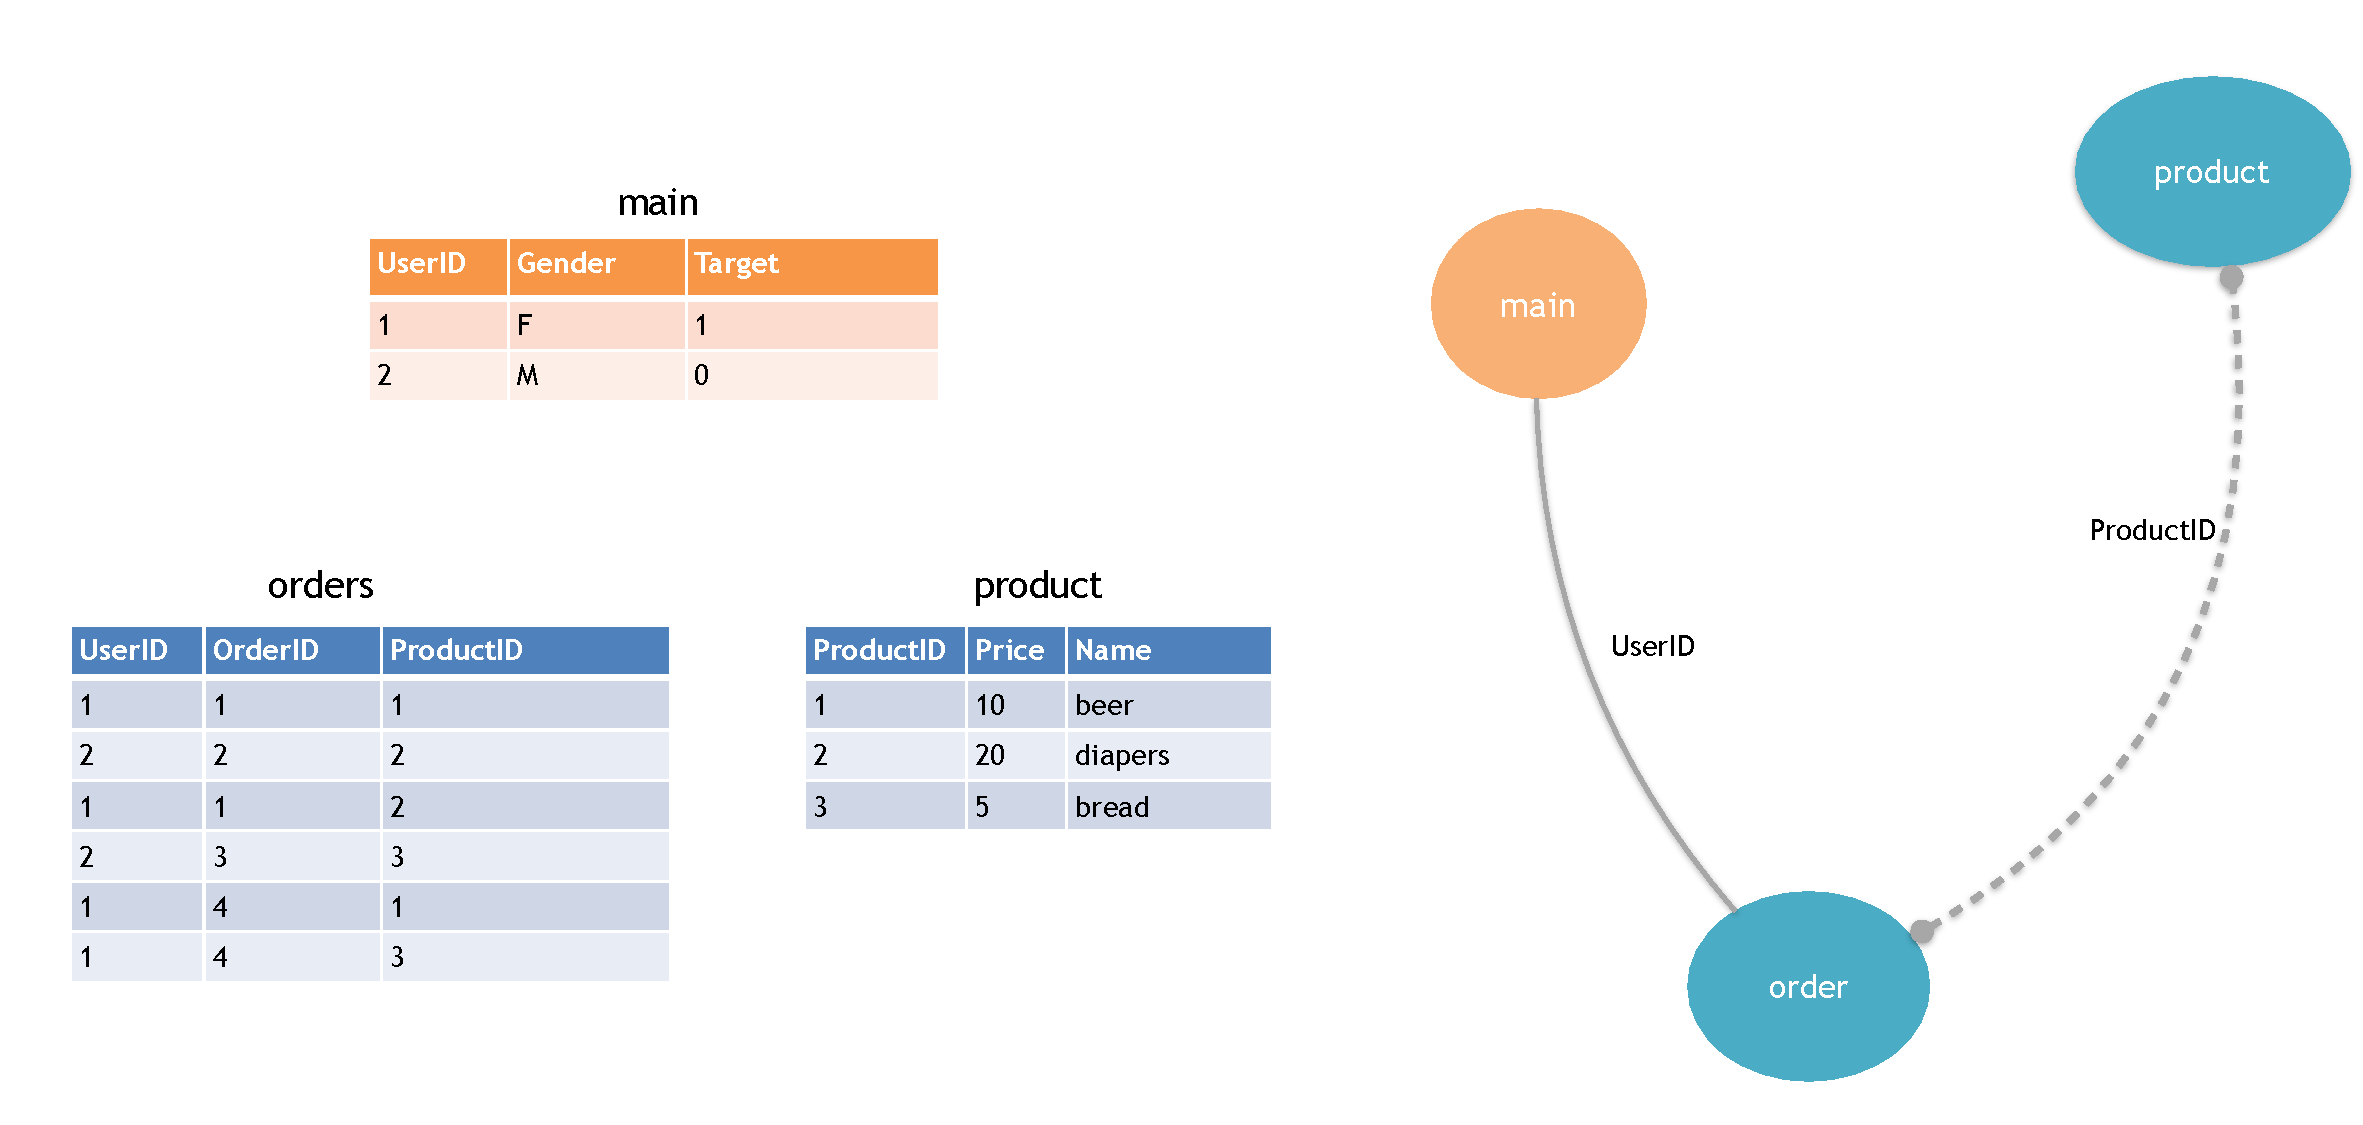
\includegraphics[width=1.0\columnwidth]{./toys.pdf}
    \caption{A toy database and its entity graph.}
    \label{fig:database}
\end{figure}


\begin{example}
Figure \ref{fig:database} shows a sample toy database with 3 tables, this simple database will be considered as a running example throughout the paper:
\begin{itemize}
\item  \textit{main}: user information with a target column indicating whether a user is a loyalty customer. Each entry in the main table is uniquely identified by the UserID column. 
\item  \textit{order}: contains user shopping information. Each order includes product identifiers that link to the product table.
\item  \textit{product}: contains information about the products such as product price and product name.
\end{itemize}
\end{example}

An entity graph is a relational graph where nodes are tables and edges are links between tables via primary/foreign key relationships. Figure \ref{fig:database} shows the entity graph of the database in the same figure.

\begin{definition} [Joining path]
A joining path is defined as a sequence $p = T_0 \xrightarrow{c_1} T_1 \xrightarrow{c_2} T_2 \cdots \xrightarrow{c_k} T_k \mapsto c$, where $T_0$ is the main table, each $T_i$ is a table in the database, $c_i$ is a foreign key column connecting tables $T_{i-1}$ and $T_i$, and $c$ is a data column (or a list of columns) in the last table $T_k$ in the path.
\end{definition}


\begin{example}
Following the joining path $p = main \xrightarrow {UserID} order \xrightarrow {ProductID} product \mapsto Price$, we can obtain the price of all products that have been purchased by a user. In this example, $c =  Price$ is a column in the last table in the joining path. However, in general, c can be any list of columns with different data types.
\end{example}




\begin{definition} [Relational tree]
Given a training example with identifier $e$ and a joining path  $p = T_0 \xrightarrow{c_1} T_1 \xrightarrow{c_2} T_2 \cdots \xrightarrow{c_k} T_k \mapsto c$, a relational tree, denoted as $t^p_e$, is a tree representation of the joined result for the entity $e$ following the joining path $p$. The tree  $t^p_e$ has maximum depth $d = k$. The root of the tree corresponds to the training example $e$. Intermediate nodes at depth $0 < j < k$ represent the rows in the table $T_j$. A node at depth $j-1$  connects to a node at depth $j$ if the corresponding rows in tables $T_{j-1}$ and table $T_j$ share the same value in the key column $c_j$. Each leaf node of the tree represents the value of the data column $c$ in the last table $T_k$.
\end{definition}

\begin{example}
\label{exp:relational tree}
Figure \ref{fig:relational tree} shows two relational trees for $UserID=1$ and $UserID=2$ following the joining path $p = main \xrightarrow {UserID} order \xrightarrow {ProductID} product \mapsto Price$. As can be seen, the first user made two orders with $OrderID = 1$ and $OrderID = 4$ represented by two intermediate nodes at depth $d=1$. Besides, order 1 includes two products with $ProductID = 1$ and $ProductID = 2$, while order 4 consists of products with $ProductID = 1$ and $ProductID = 3$. The leaves of the tree carry the price of the purchased products.
\end{example}

\begin{figure}[tb]
    \centering
    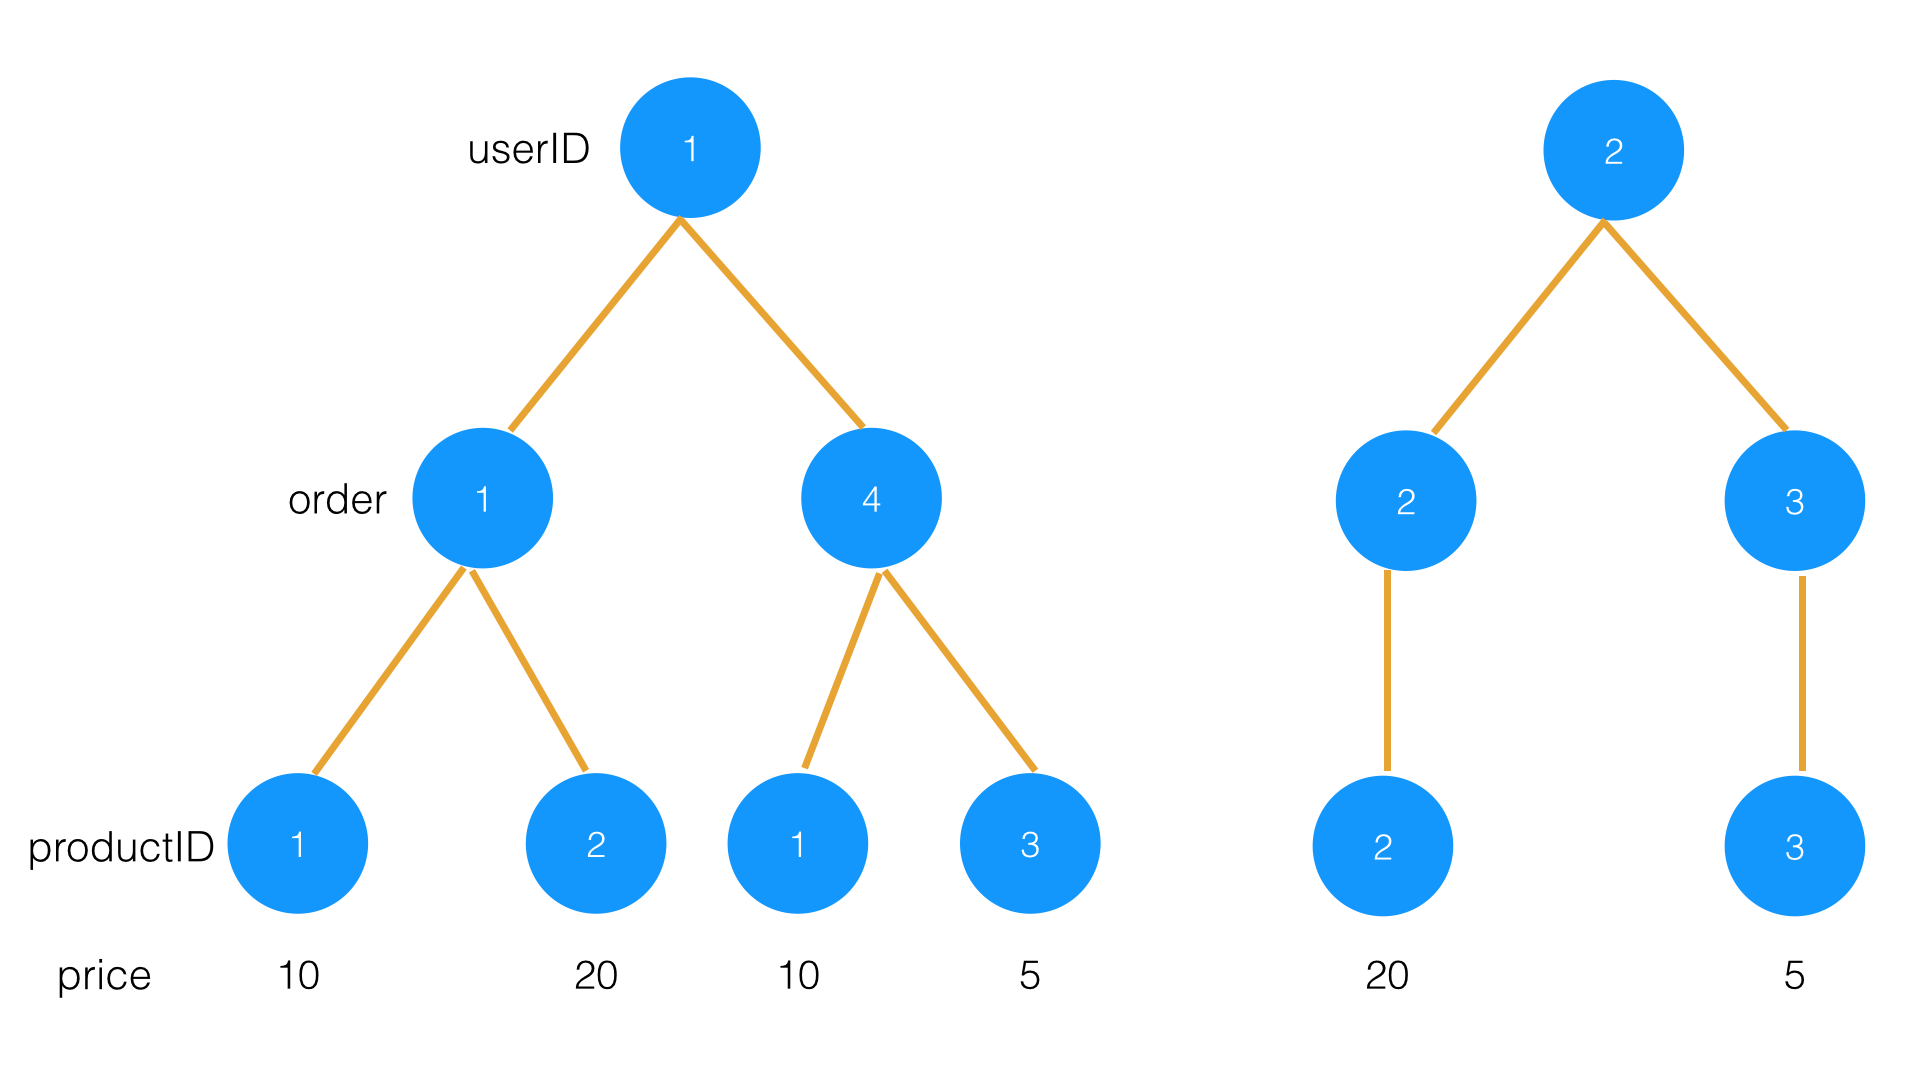
\includegraphics[width=1.0\columnwidth]{./rtree.png}
    \caption{Relational trees: $t^p_1$ (left) and $t^p_2$ (right).}
    \label{fig:relational tree}
\end{figure}

\begin{definition} [Transformation function]
Given a relational tree $t^p_e$, a transformation function $f$ maps a relational tree $t^p_e$ to a fixed size  vector $x \in R^l$, i.e. $f(t^p_e) = x$. Vector $x$ is called a feature vector.
\end{definition}


\section{Problem definition}


Let $D_p = \{t^p_1, t^p_2, \cdots, t^p_m\}$ be the set of all relational trees collected for all training examples in the database following the joining path $p$ . In the database $D$, each training example is associated with a label, therefore, for each $D_p$,  we have a target set denoted as $Y = \{y_1, y_2, \cdots, y_m\}$, where the target variable $y_i$ is associated with $t^p_i$. Denote $x_i$ as the feature vector obtained from the relational tree $t^p_i$ by transformation $f$, i.e. $x_i = f(t^p_i)$, therefore, from $D_p$ we can obtain $X = \{x_1,x_2, \cdots, x_m\}$, i.e. a set of feature vectors.

\begin{definition} [Prediction function]
Given a set of feature vectors $X = \{x_1, x_2, \cdots, x_m\}$, a function $g$ mapping every feature vector $x_i$ to an estimate value $\hat{y}_i$, which approximates $y_i$, is called a prediction function for the target set $Y$.
\end{definition}


The prediction function $g$ approximates the target set $Y$ by a set of estimates $\hat{Y} = \{\hat{y}_1, \hat{y}_1, \cdots, \hat{y}_m\}$. Let $L_{f,g}(Y, \hat{Y})$ denote the loss function that represents the prediction error when the raw data is transformed by the transformation function $f$ and the target variable is predicted by the prediction function $g$. The feature learning problem can be formulated as follows:   
\begin{problem}[Feature learning for a joining path]
\label{prob:Feature learning for a joining path}
Given a joining path $p$ and the set of  relational trees  $D_p = \{t^p_1, t^p_2, \cdots, t^p_m\}$ collected for the training examples following the path $p$, find the transformation and prediction functions $f^*$ and $g^*$ such that $f^*, g^* = argmin L_{f,g}(Y,\hat{Y})$
\end{problem}

Problem \ref{prob:Feature learning for a joining path} is defined for each individual joining path $p$. In general, we can define  a feature learning problem for an entire set of joining paths generated from the entity graph. Denote $P =\{p_1,p_2,\cdots,p_q\}$ as a set of joining paths extracted from the entity graph, $D_{p_i} = \{t^{p_i}_1, t^{p_i}_2, \cdots, t^{p_i}_m\}$ as the set of relational trees corresponding to the path $p_i$. Let $f_{p_i}$ be a transformation function that transforms each element of $D_{p_i}$ into an element of the feature vector set $X_i = \{x^i_1, x^i_2, \cdots, x^i_m\}$. Let $g$ be a prediction function that takes as input $x^1_j \oplus x^2_j \oplus \cdots \oplus x^q_j $, for $j = \overline{1,m}$, and produces an estimate $\hat{y}_j$ of $y_j$, where $\oplus$ stands for the vector concatenation operator.

\begin{problem}[Feature learning]
\label{prob:Feature learning}
Given a collection of joining paths  $P =\{p_1,p_2,\cdots,p_q\}$ and the corresponding relational tree sets  $\{D_{p_1}, D_{p_2}, \cdots, D_{p_q} \}$, find the transformation and prediction functions $f^*$ and $g^*$ such that $f^*, g^* = argmin L_{f,g}(Y,\hat{Y})$.
\end{problem}

Problems \ref{prob:Feature learning for a joining path} and \ref{prob:Feature learning} are similar, except that the loss function is jointly optimized in Problem \ref{prob:Feature learning}. Solving Problem \ref{prob:Feature learning for a joining path} for each joining path may result in a set of redundant features because similar paths produce only slightly different relational trees. On the other hand, solving problem \ref{prob:Feature learning} may result in a more compact set of features but the optimization problem is more complicated.


\section{A rule based approach}
Given relational trees, there are different ways to transform the trees into features. In this section, we discuss rule-based approaches that define several transformation functions based on heuristics. The method discussed in this section is an extension of the Data Science Machine (DFS) \cite{DFS} so we first briefly recall the DFS algorithm.

\begin{figure}[tb]
    \centering
    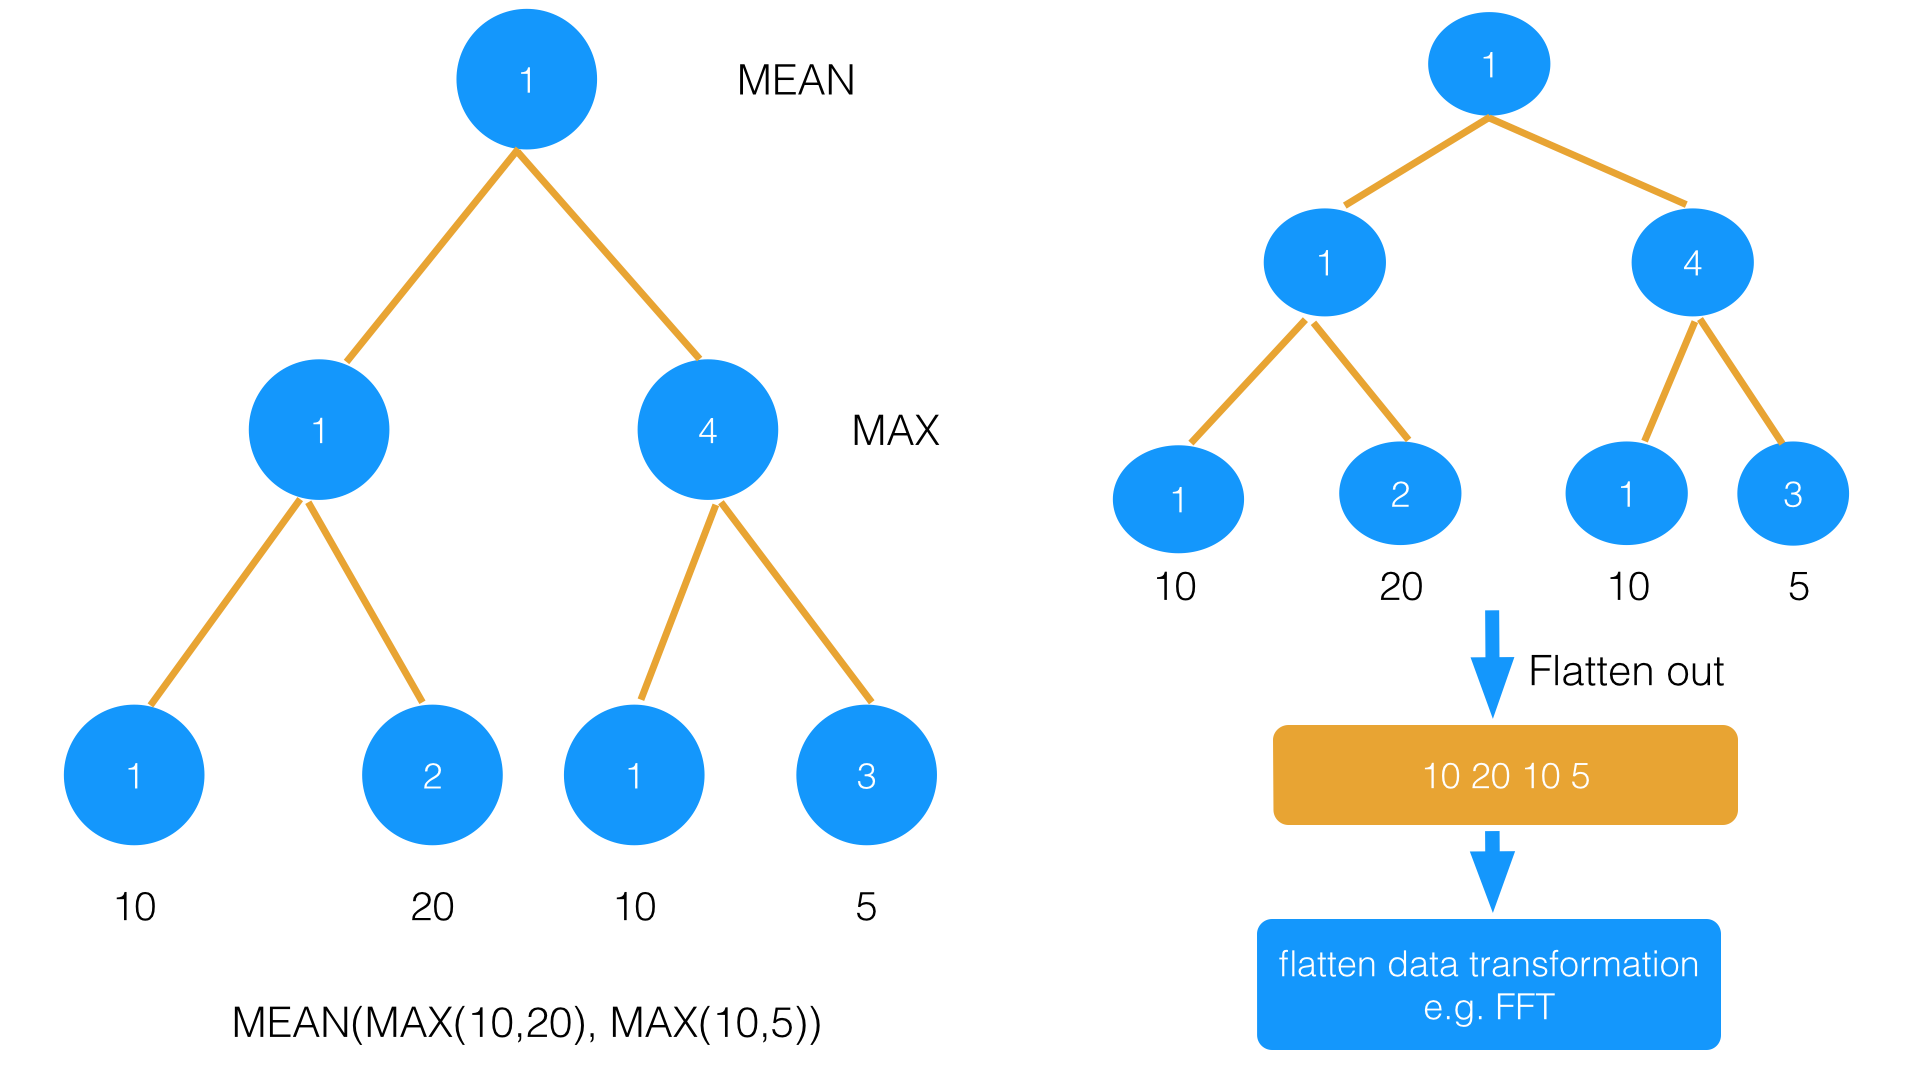
\includegraphics[width=1.0\columnwidth]{./prior_art.png}
    \caption{Prior arts on relational trees transformation: DFS uses augmented aggregation functions at each level of the tree (left). On the other hand, OneBM flattens out the trees and transforms the flattened results using transformations that support unstructured and with temporal ordered data.}
    \label{fig:relational tree transformation prior art}
\end{figure}


In the Data Science Machine (DFS) \cite{DFS}, transformation function $f$ is a composition of basic aggregation functions such as AVG, SUM, MIN and MAX augmented at each level of a tree. For instance, for the relational tree $t^p_1$ in Figure \ref{fig:relational tree}, a feature can be collected for $UserID=1$ as can be seen in Figure \ref{fig:relational tree transformation prior art} (left) by applying the aggregation functions at each level of the tree. The aggregation function takes input from the node's children and outputs a value served as input to its parent. The example on Figure \ref{fig:relational tree transformation prior art} (left) produces a feature $AVG(MAX(10,20),MAX(10,30)) = 25$ which corresponds to the average of the maximum price of products purchased by the user with $UserID=1$. 



DFS worked well for numerical data, however, when the data at the leaves of the trees are categorical or unstructured data such as texts, simple aggregations do not apply. Moreover, when the nodes of the trees have orders the trees carry sequences or time-series which is not easily handled in the DFS framework. Therefore, we extend DFS to One Button Machine (OneBM) in an unpublished manuscript \cite{onebm} to deal with such situation. 

In OneBM, the tree is first flattened out by a GroupBy operation at the root node to produce a set or a sequence of values. Depending on the type of the values carried at the leaves, different transformations are applied. For instance, for the tree $t^p_1$ in Figure \ref{fig:relational tree}, the tree can be flattened out into a multi-set: $s = \{10, 30, 10, 20\}$ as can be seen on Figure \ref{fig:relational tree transformation prior art} (right). When there are orders associated the values carried at leaves, the multi-set is turned into a timeseries. In that case, popular timeseries based features are extracted from $s$ such as the autoregressive coefficients or the coefficients of Fast Fourier Transformation. A full list of transformations for each special type of data is described in Table \ref{tab:rules}, the list covers most of important data type of the flattened trees.

\begin{table}
  \caption {Transformation rules in OneBM} \label{tab:rules} 
  \begin{tabular}{ | l | c | }
    \hline
    \textbf{Data type} & \textbf{transformation functions} \\ \hline
    numerical &  as is  \\ \hline
    categorical & order by frequency and \\
    & use order as the transformation  \\ \hline
    text & see sequence features \\ \hline
    timestamp & calendar features, gap to cut-off time if exists \\ \hline
    timestamp series & series of gaps to cut-off time if exists \\ \hline
    number multi-set & avg, variance, max, min, sum, count \\ \hline
    set of texts & see sequence features \\ \hline
	multi-set of items & count, distinct count, \\ & high correlated items \\ \hline
	timeseries &  avg, max, min, sum, count, variance, \\ &recent($k$), normalized count and \\ & sum to the max gap to cut-off   \\ \hline
	sequence & count, distinct count, \\& high correlated symbols \\ 
    \hline
  \end{tabular}
\end{table}

Once features are generated by the given set of rules, feature selection is needed to remove irrelevant features. We used statistical hypothesis test to remove leak features (distribution is different on validation and training sets) \cite{onebm}. Besides, we filtered out irrelevant features with very low correlation in regression problems or very low information gain in classification problems.


\section{Learning features}
The rule based approaches specify the transformation functions based on heuristics regardless of the domain. In practice, a predefined transformation function can't be universally relevant for any use-case. Therefore, in this section we will discuss an approach that searches for transformations via supervised learning. In other words, the transformations are learned from the data rather than being specified \textit{a-priori} by the user.
\subsection{Relational recurrent neural network}
\label{sec:r2n}
To simplify the discussion, we make some assumptions as follows (an extension to the general case is discussed in the next section):
\begin{itemize}
\item the last column $c$ in the joining path $p$ is a fixed-size real number vector 
\item all nodes at the same depth of the relational tree are ordered according to a predefined order
\end{itemize}

With the given simplification, transformation function $f$ and prediction function $g$ can be learned from data by training a deep neural network structure that includes a set of recurrent neural networks (RNNs). We call the given network structure \textit{relational recurrent neural network} (r2n) as it transforms relational data using recurrent neural networks.

There are many variants of RNN, in this work we assume that an RNN takes as input a sequence of vectors and outputs a vector. An RNN is denoted as $rnn(s, \theta)$, where $s$ is a variable size sequence of vectors and $\theta$ is the network parameter. Although the discussion focuses on RNN cells, our framework also works for Long Short Term Memory (LSTM) or Gated Recent Unit (GRU) cells.


\begin{definition} [Relational Recurrent Neural Network]
For a given relational tree $t^p_e$, a relational recurrent neural network is a function denoted as $r2n (t^p_e, \theta)$ that maps the relational tree to a target value $y_e$. An $r2n$ is a tree of $RNNs$, in which at every intermediate node, there is an $RNN$ that takes as input a sequence of output vectors of the $RNNs$ resident at its children nodes. In an $r2n$, all RNNs, resident at the same depth $d$, share the same parameter set $\theta_d$. If the maximum depth of the tree $t^p_e$ is $k$, there are overall $k$ sets of parameters in the $r2n$ encoded as $\theta = \{\theta_1, \theta_2, \cdots, \theta_k\}$.
\end{definition}

\begin{example}
\label{exp:r2n}
  Figure \ref{fig:r2n} shows two unfolded relational recurrent neural networks for the relational trees described in Figure \ref{fig:relational tree}. As it is observed, an $r2n$ summarizes the data under every node at depth $d$ in the relation tree via a function parametrized by an RNN with parameters $\theta_d$.
\end{example}

Since $RNN$ is a universal model \cite{universal}, that approximates any function which can be calculated by a Turing machine, the given proposed $r2n$ can approximate the functions specified in DFS and OneBM as well. 
\begin{figure}[tb]
    \centering
    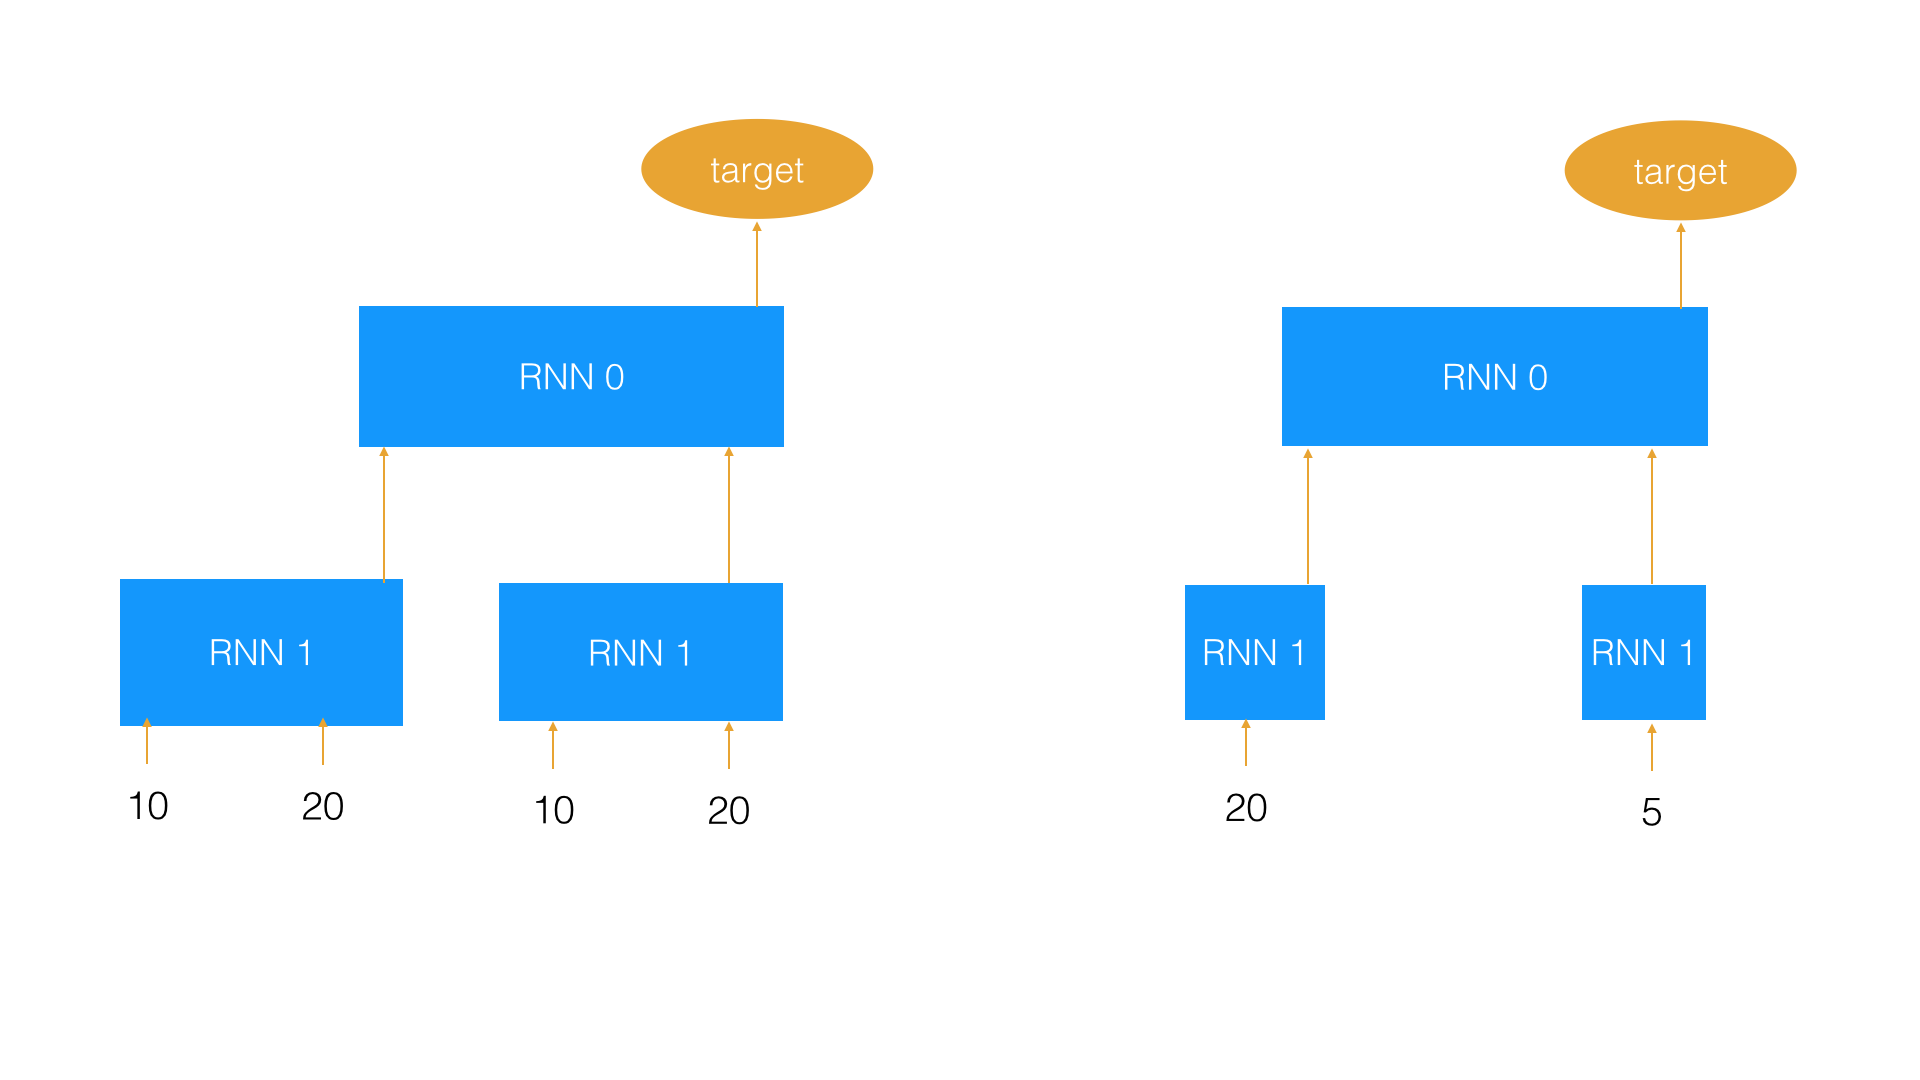
\includegraphics[width=1.0\columnwidth]{./r2n.png}
    \caption{Unfolded r2n neural networks for the relational trees in Figure \ref{fig:relational tree}.}
    \label{fig:r2n}
\end{figure}   
\subsection{A universal r2n}
\label{sec:r2n universal}
In this section, we discuss a neural network structure that works for the general case even without the two assumptions made in Section \ref{sec:r2n}. 

\subsubsection{Dealing with unstructured data}
Regarding the first assumption, we add at each leaf node an embedding layer that embeds the input value to a vector of numerical value regardless of the type of the input. The embedded vectors can be learned jointly with the $r2n$ network as shown in Figure \ref{fig:universal r2n}. We call the given network structure a universal $r2n$ network. For example:
\begin{itemize}
\item if the input value is a categorical value, a direct look-up table is used that map each categorical value to a fixed size vector. 
\item if the input is a sequence, including a sentence or a symbolic sequence, an RNN is used to learn a sequence embedding.
\item if the input is an image, a convolution net is used to learn an image embedding.
\item if the input is a timeseries, an RNN is used to learn a timeseries embedding.
\item if the input is a GPS trajectory, an RNN is used to learn an embedding. 
\item if the input is an itemset, an order is defined over the set and the set is treated as a sequence 
\item if the input is a graph, a graph embedding algorithm is used 
\end{itemize}
\begin{figure}[tb]
    \centering
    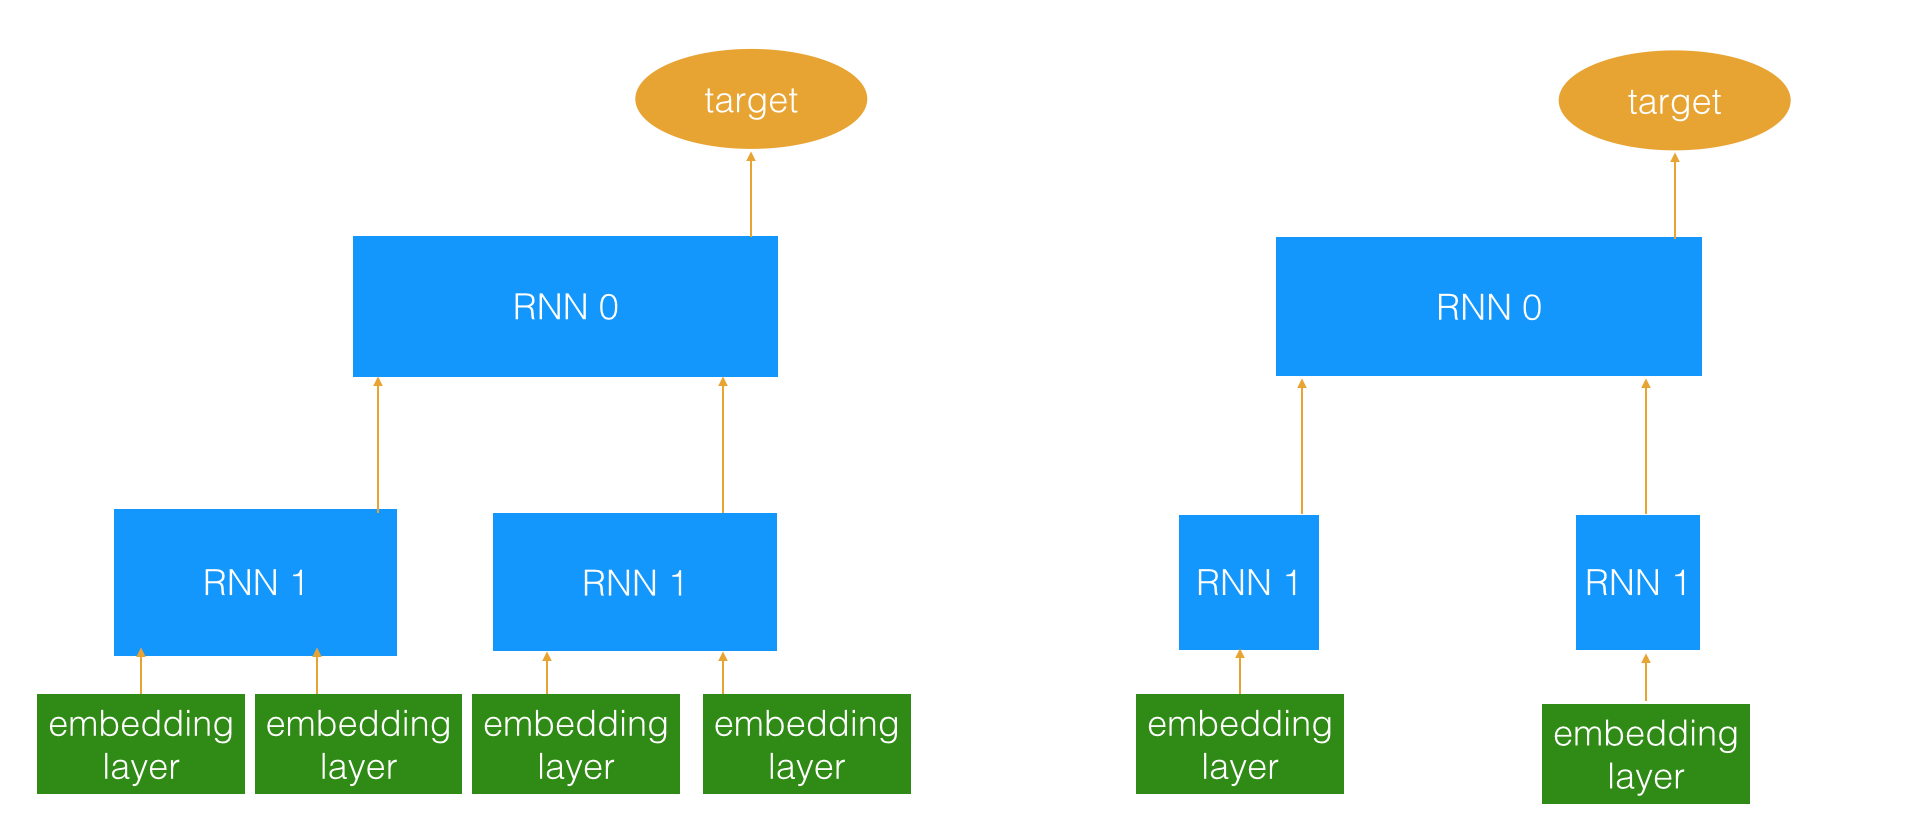
\includegraphics[width=1.0\columnwidth]{./er2n.png}
    \caption{Universal r2n neural networks for the relational trees in Figure \ref{fig:relational tree}. Embedding layers transform unstructured data to numerical data before input to the r2n.}
    \label{fig:universal r2n}
\end{figure}
In principle, the given list can be extended to handle more complicated data types such as a sequence of sequences and a set of images. In any cases, the key components of the universal $r2n$ always consists of an $r2n$ and a data embedding structure under every leaf node of the $r2n$.
\subsubsection{Dealing with unordered data}
When the children nodes under a node in the relational tree are not associated with an order, the input to the recurrent neural network at the given node is a set instead of a sequence. In that case, the transformation function we need to build is a function $f(s)$ that maps from an input set of numerical vectors to an output numerical vector, we call such function as set transformation. It is important to notice that, $s$ is a set of vectors, and $f(s)$ is invariant in any random permutation of $s$. 
In order to use recurrent neural networks as an approximation of $f(s)$, we can randomly permute the order of $s$ before transforming the set of the network. An interesting question to ask is whether or not recurrent neural network can be used to approximate any set function $f(s)$. Unfortunately, the following theorem shows that, there is no recurrent neural network that can approximate any set function except the constant or the sum function.
\begin{lemma}
A recurrent neural network $rnn(s, W, H, U)$ with linear activation is a set function if and only if $H=1$ or $rnn(s, W, H, U)$ is a constant.
\label{lemma:set function rnn}
\end{lemma} 
\begin{proof}
Due to space limit, proof is moved to appendix.
\end{proof}

 
 \begin{theorem}
If a recurrent neural network $rnn(s, W, H, U)$ with linear activation is a set function, it is either a constant function or can be represented as: 
\begin{eqnarray}
rnn(s, W, H, U) &=& c + h_0U + |s|*bU + UW*sum(s) 
\label{eq:rnn set}
\end{eqnarray}
\end{theorem} 
\begin{proof}
According to Lemma \ref{lemma:set function rnn}, $rnn(s, W, H, U)$ is either a constant function or $H=1$. Replace $H = 1$ to the formula of an RNN we can easily obtain equation \ref{eq:rnn set}.
\end{proof}
From equation \ref{eq:rnn set} we can see that the set of functions that an rnn network can approximate is limited. It is straightforward to show that the function in equation \ref{eq:rnn set} does not include the Max and Min function. The key issue is originated from the fact that the input to the RNN doesn't have an order. Fortunately, we can go around the given issue by defining  an artificial order for the data, e.g. by sorting them according to a statistics related to the data. In particular, if the data is a vector of numerical value, we order the data according to the mean value of the vector elements or the data is order by the primary key column in the table where the data is collected from. One important thing we should guarantee is that the order must be kept consistent across training/test data.

 \subsection{Joining path generation}
 So far we have discussed feature learning from relational trees extracted from a database when a joining path is given. In this section, we discuss different strategies to generate relevant joining paths. Recall that the input to our system is a relational database with multiple tables. From the database we create an entity graph where nodes correspond to database tables and edges are foreign key relations between tables. A joining path always starts from the main table following a graph traverse strategy to be defined later in this section. First, we discuss the hardness of finding a relevant path for a given predictive analytics problem in the following theorem.
\begin{figure}[tb]
    \centering
    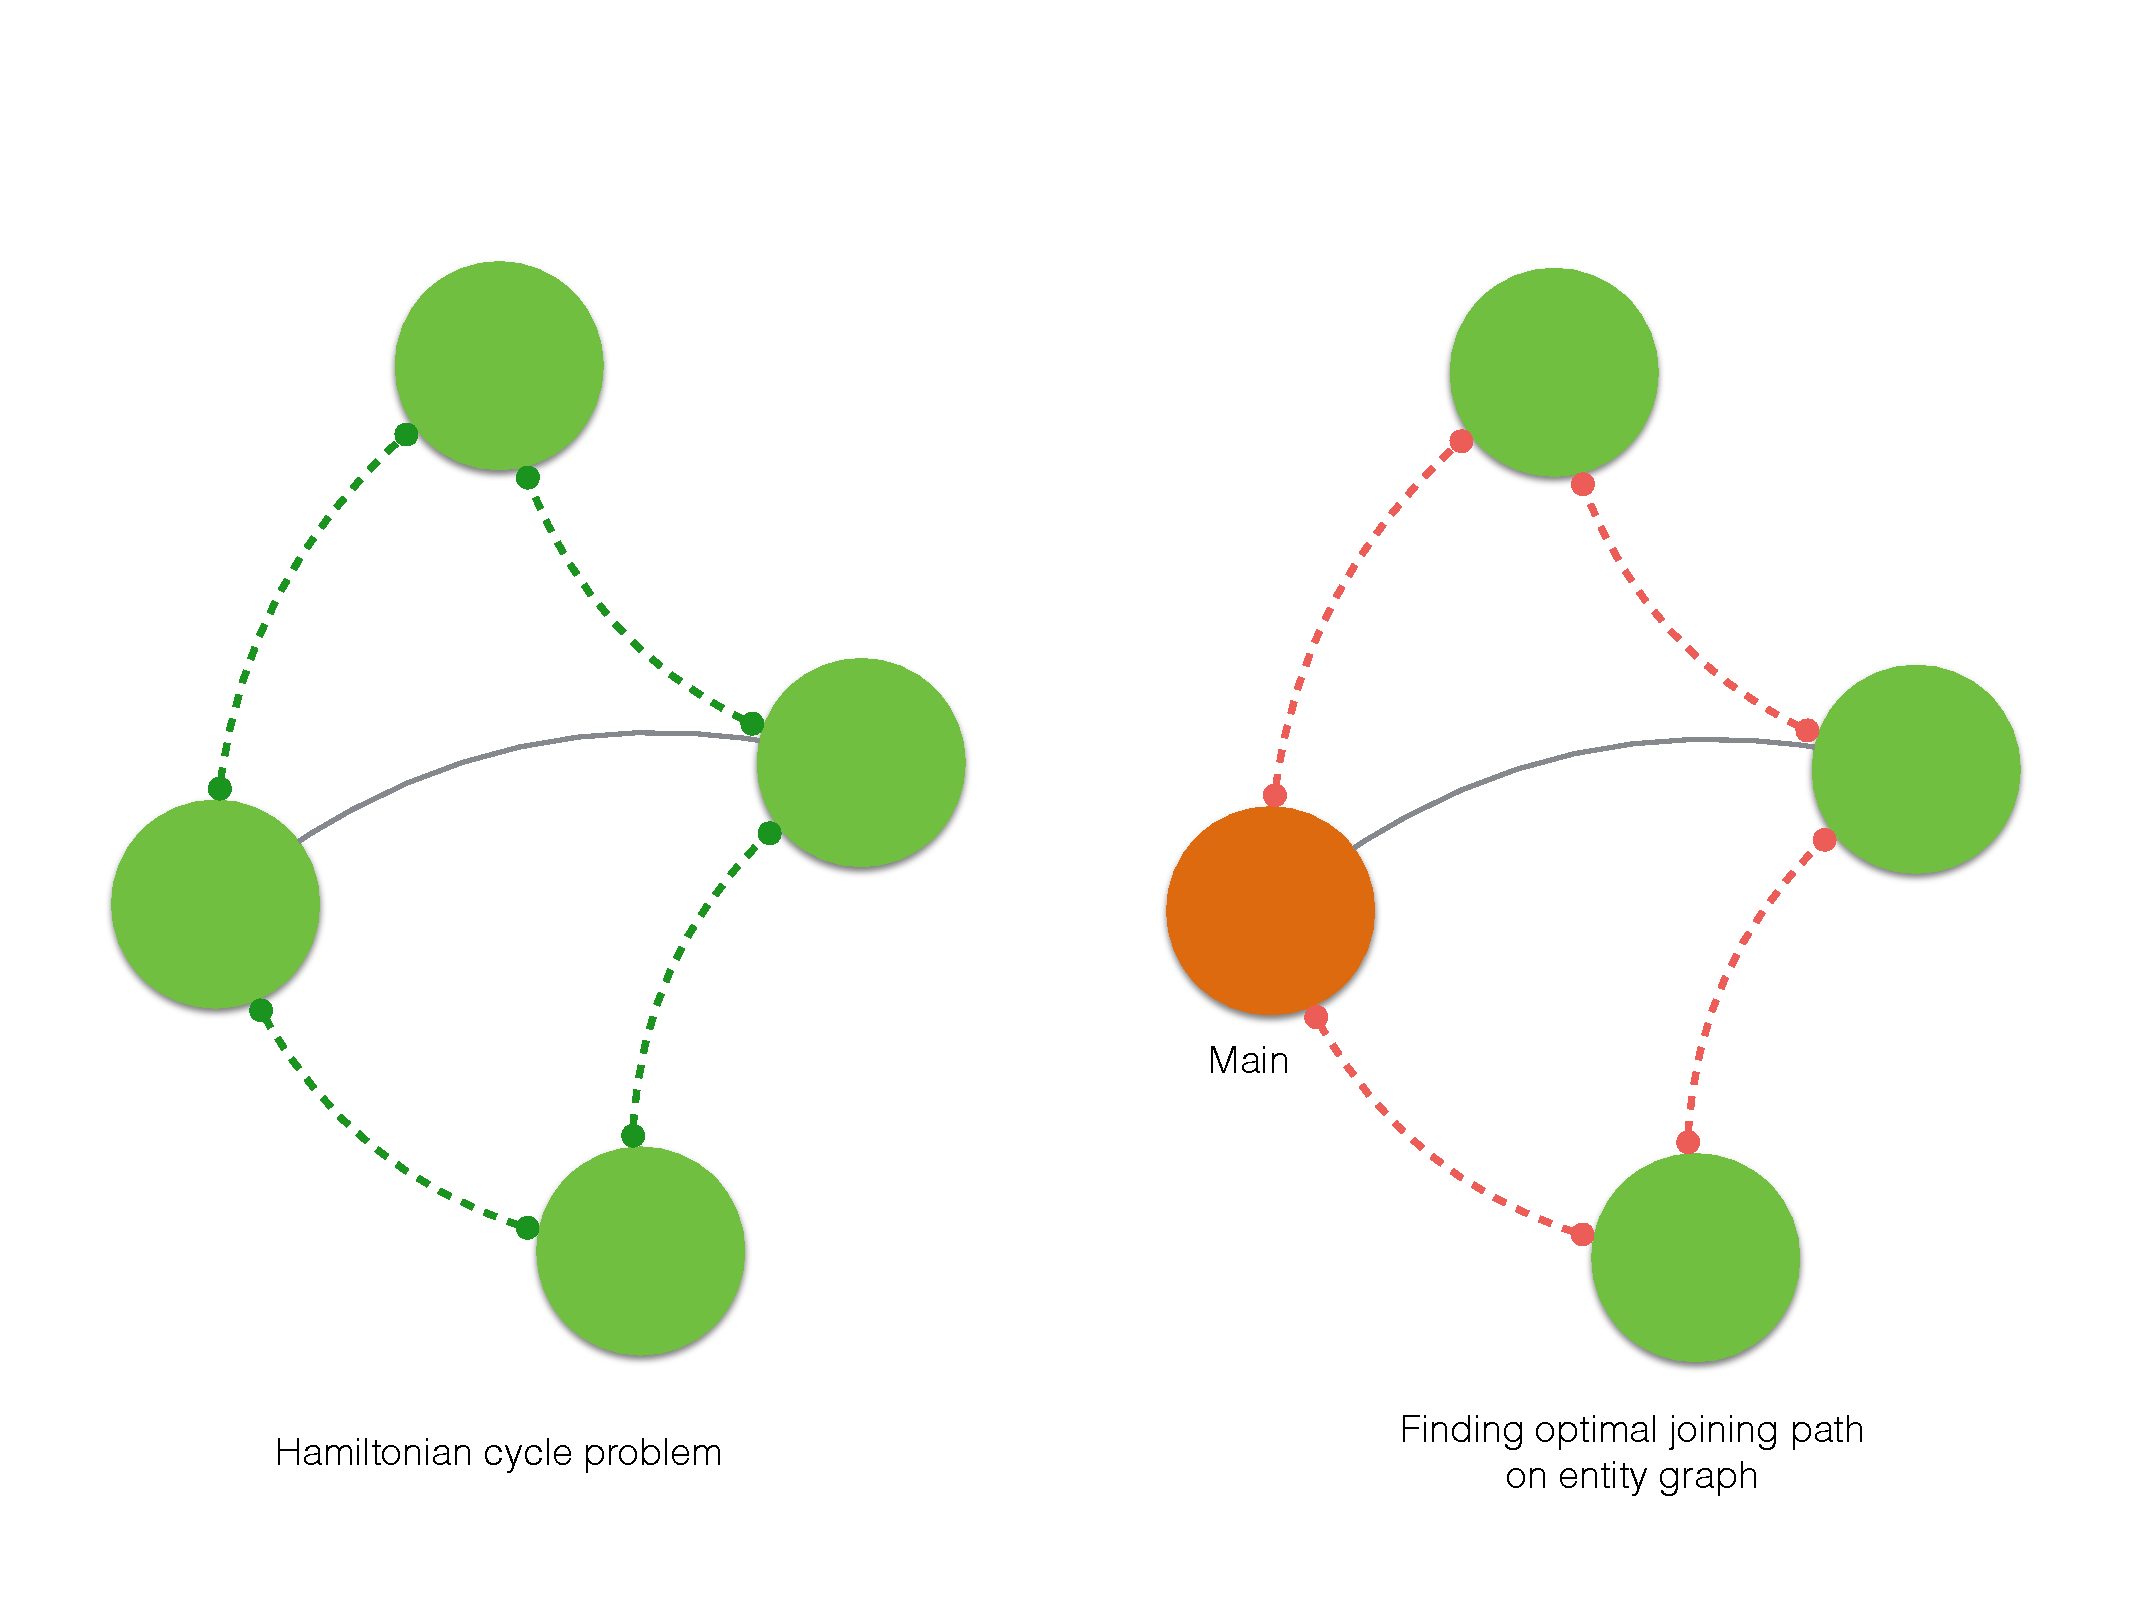
\includegraphics[width=1.0\columnwidth]{./hamilton.pdf}
    \caption{A reduction from Hamiltonian cycle problem to the problem finding the optimal joining path for engineering features from relational data for a given predictive analytics problem.}
    \label{fig:np-hardness}
\end{figure}  
 
\begin{theorem}
Given an entity graph, searching for the relevant path to extract features from the entity graph for predicting the correct label of the main table entries is an NP-Hard problem.
\end{theorem} 
\begin{proof}
We prove the NP-hardness by reduction to the \textit{Hamiltonian cycle problem} which was well-known as an NP-Complete problem \cite{karp1972reducibility}. Given a graph $G(E,V)$, where $E$ is a set of undirected edges and $V$ is a set of nodes. The Hamiltonian cycle problem asks if there exists a cycle on the graph such that there is no node visited twice in the cycle.

Given an instance of the Hamiltonian cycle problem, we create an instance of a predictive analytics problem with an entity graph as demonstrated in Figure \ref{fig:np-hardness}. We assume that we have a database $D$ with $|V|$ tables, each table corresponds to exactly one node in $|V|$. For each edge in $ (n_1, n_2 \in E)$, there is a foreign key that connects two tables associated with nodes $n_1$ and $n_2$.

Therefore, the entity graph of $D$ is an isomorphism to  $G(E,V)$. For each training instance $t$, depending on the joined results, there is a subgraph $g_t \in G$ from which we can generate features to predict the target value of $t$ following any joining path in $g_t$.

Assume that our interested predictive analytics problem is a binary classification problem in which $t$ has a positive label if and only if there is a Hamiltonian cycle in $g_t$. If we choose an instance $t$ such that $g_t = G$, predicting the label of $t$ is equivalent to determining if there is a Hamiltonian cycle in $g_t$. Therefore, solving the feature engineering problem, we have a solution to the Hamiltonian cycle problem from which the theorem is proved.
\end{proof}

Because finding the optimal path is hard, we limit the maximum depth of the joining paths and propose simple strategies for efficient traversing the graphs. As can be seen in experiments, these strategies cover the most important paths in practice and produce high quality features. Particularly, our system supports three different graph traversal strategies:
\begin{itemize}
\item simple: only allows simple paths (no repeated nodes)
\item forward only: nodes are assigned depth numbers based on a breadth-first traversal starting from the main table. Path generation only considers the paths such that latter nodes  must be deeper than the former ones.
\item all: all paths are considered
\end{itemize} 

In our experiments, forward only is the most efficient which is our first choice. The other strategies are supported for the completeness. For any strategy, the joined tables can be very large, especially when the maximum depth is set high. We apply sampling strategies and caching intermediate tables to save memory and speed up the join operations. Details on these techniques can be found in our manuscript on arxiv \cite{onebm}.

\subsection{Networks for multiple joining paths}
This section discusses the network structure for learning features from multiple joining paths. Recall that for each joining path $p_i$, we create an $r2n_i$ network that learns features from the data generated by the joining path. In order to jointly learn features from multiple joining paths ${p_1,p_2,\cdots,p_m}$, we use a fully connected layer that connects the output of the RNN network at the root nodes of the $r2n_i$ to a fixed size output vector for all r2n networks. Consequently, we concatenate these vectors and use a feed-forward network with several hidden layers with desired final output size. 
\begin{figure}[tb]
    \centering
    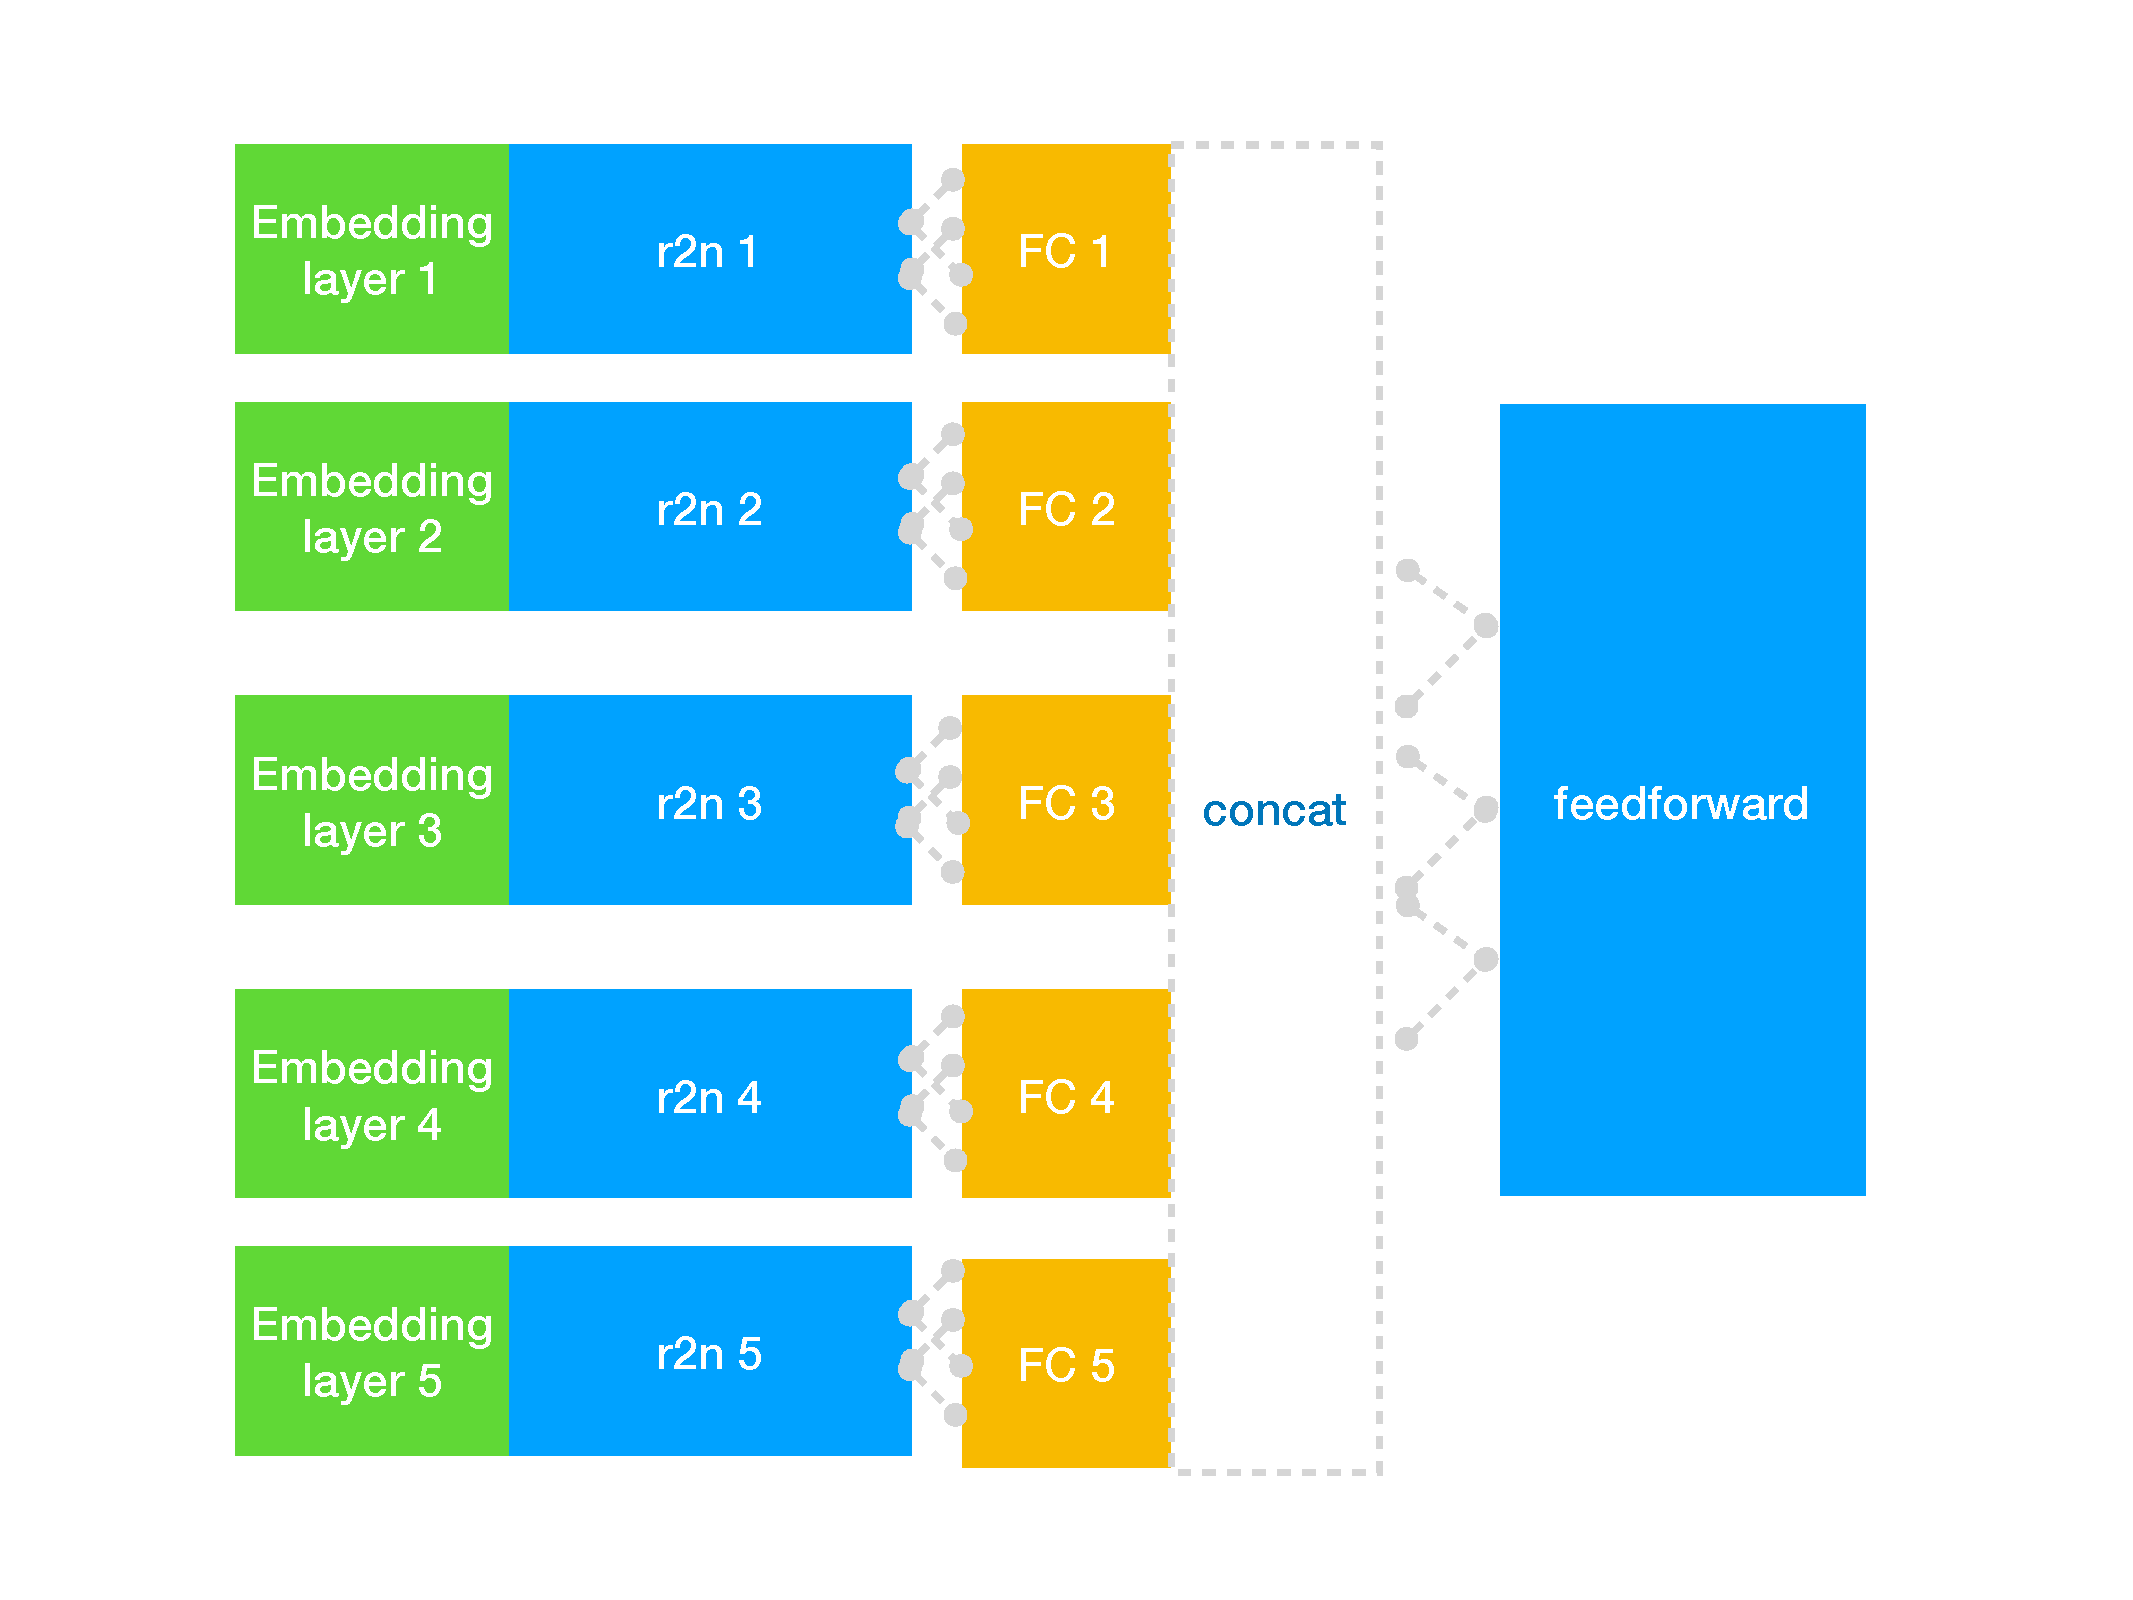
\includegraphics[width=1.0\columnwidth]{./bigr2n.pdf}
    \caption{Feature learning from multiple joining paths. Data collected by each joining path is transformed using an optional embedding layer, a r2n network and a fully connected layer (FC) consecutively. The outputs of the FCs are concatenated and transformed again by a feedforward layer.}
    \label{fig:bigr2n}
\end{figure}  
 
For regression problems, the final output size is a scalar value. For classification problems, the final output size is a vector with size equal to the number of classes. Besides, a softmax function is applied on the final output vector to obtain the class prediction distribution for classification problem. The entire network structure is illustrated on Figure \ref{fig:bigr2n}. Training the given network is done via the standard back-propagation algorithm.
   
\section{Experiments}
In this section we discuss the experimental setup and our results. We start by detailing the data and the required preprocessing steps.
Finally, we compare our work to the DFS method, which is considered as the state-of-the-art of automatic feature engineering for relational data, on the data of three different Kaggle challenges.  Due to space limit, more details about parameter settings and set-up for the baseline methods can be found in Appendix. 
\subsection{Datasets preparation}
\begin{table}
  \caption {Dataset size} \label{tab:data size} 
  \begin{tabular}{ | l | c | l | c |}
    \hline
    \textbf{Data} & \textbf{$\sharp$ tables} & \textbf{$\sharp$ columns} & \textbf{size} \\ \hline
    KDD Cup 2014 & 4 & 51 & 0.9  GB \\ \hline    
    Coupon purchase &  7 &  50 & 2.2 GB   \\ \hline 
    Grupo Bimbo &  5 &  19 & 7.2 GB   \\ \hline        	
  \end{tabular}   
  \caption{Datasets used in experiments.} 
\end{table}

The following data preparation steps are needed to turn the raw data into the format that our system requires:
\begin{enumerate}
\item For every dataset we need to create a main table with training instances.  The main table is constructed  based on a very simple but practical principle: the training data must reflect exactly how the test data was created. This ensures the consistency between training and test settings.  
\item Users need to explicitly declare the database schema. 
\item Entries in a table usually represent an entity of interests, e.g. a pair of user and coupon. Each entity is identified by a key column. We added additional key columns to represent those entities if the keys are missing in the original data. 
\end{enumerate}

It is important to notice that, among three basic data preparation steps, the first one is an obligation for all Kaggle participants.  The second step is trivial as it only requires to declare the table column's special types and primary/foreign key columns. Basic column types such as numerical, boolean, timestamps, categorical etc.,  are automatically determined by our system. The last step requires  knowledge about the data but time spent on creating additional key columns is negligible compared to creating hand-crafted features.
  
\subsection{Dataset description}
\paragraph{Grupo Bimbo} participants were asked to predict weekly sales of fresh bakery products on the shelves of over 1 million stores across Mexico. The database contains 4 different tables:
\begin{itemize}
\item \textit{sale series}: the sale log with weekly sale in units of fresh bakery products. Since the evaluation is based on Root Mean Squared Logarithmic Error (RMSLE), we take the logarithm of the demand.
\item \textit{town state}: geographical location of the stores
\item \textit{product}: additional information, e.g. product names
\item \textit{client}: information about the clients
\end{itemize} 
The historical sale data spans from week 1-9 while the test data spans from weeks 10-11. We created the main table from the sale series table with data of the weeks 8-9. Data of prior weeks was not considered because there was a shortage of historical sales for the starting weeks. The main table has a target column which is the demand of the products and several foreign key columns and some static attributes of the products. 

\paragraph{Coupon Purchase} participants were asked to predict the top ten coupons which were purchased by the users in the test weeks. The dataset includes over one year of historical logs about coupon purchases and user activities: 
\begin{itemize}
\item \textit{coupon list}: static information about the coupon such as location, discount price and the shop information
\item \textit{coupon detail}: more detailed information about the coupons
\item \textit{coupon area}: categorical information about the coupon types and its display category on the website
\item \textit{coupon visit}: very large historical user activities on the coupon websites. We concatenated the user and coupon keys to create a user-coupon key that represents the user-coupon pair which is the target entity of our prediction problem.
\item \textit{user}: demographic information about the users
\item \textit{prefecture}: geographical information about the coupon and user location
\end{itemize} 
We cast the recommendation problem into a classification problem by creating a main table considering 40 weeks of data before the testing week. To ensure that the training data is consistent with the test data, for each week, we find coupons with released date falling into the following week and create an entry in the main table for each user-coupon pair. We label the entry as positive if the coupon was purchased by that user in the following week and negative otherwise. The main table has three foreign keys to represent the coupons, the users and the user-coupon pairs. 

\begin{figure*}[tb]
    \centering
    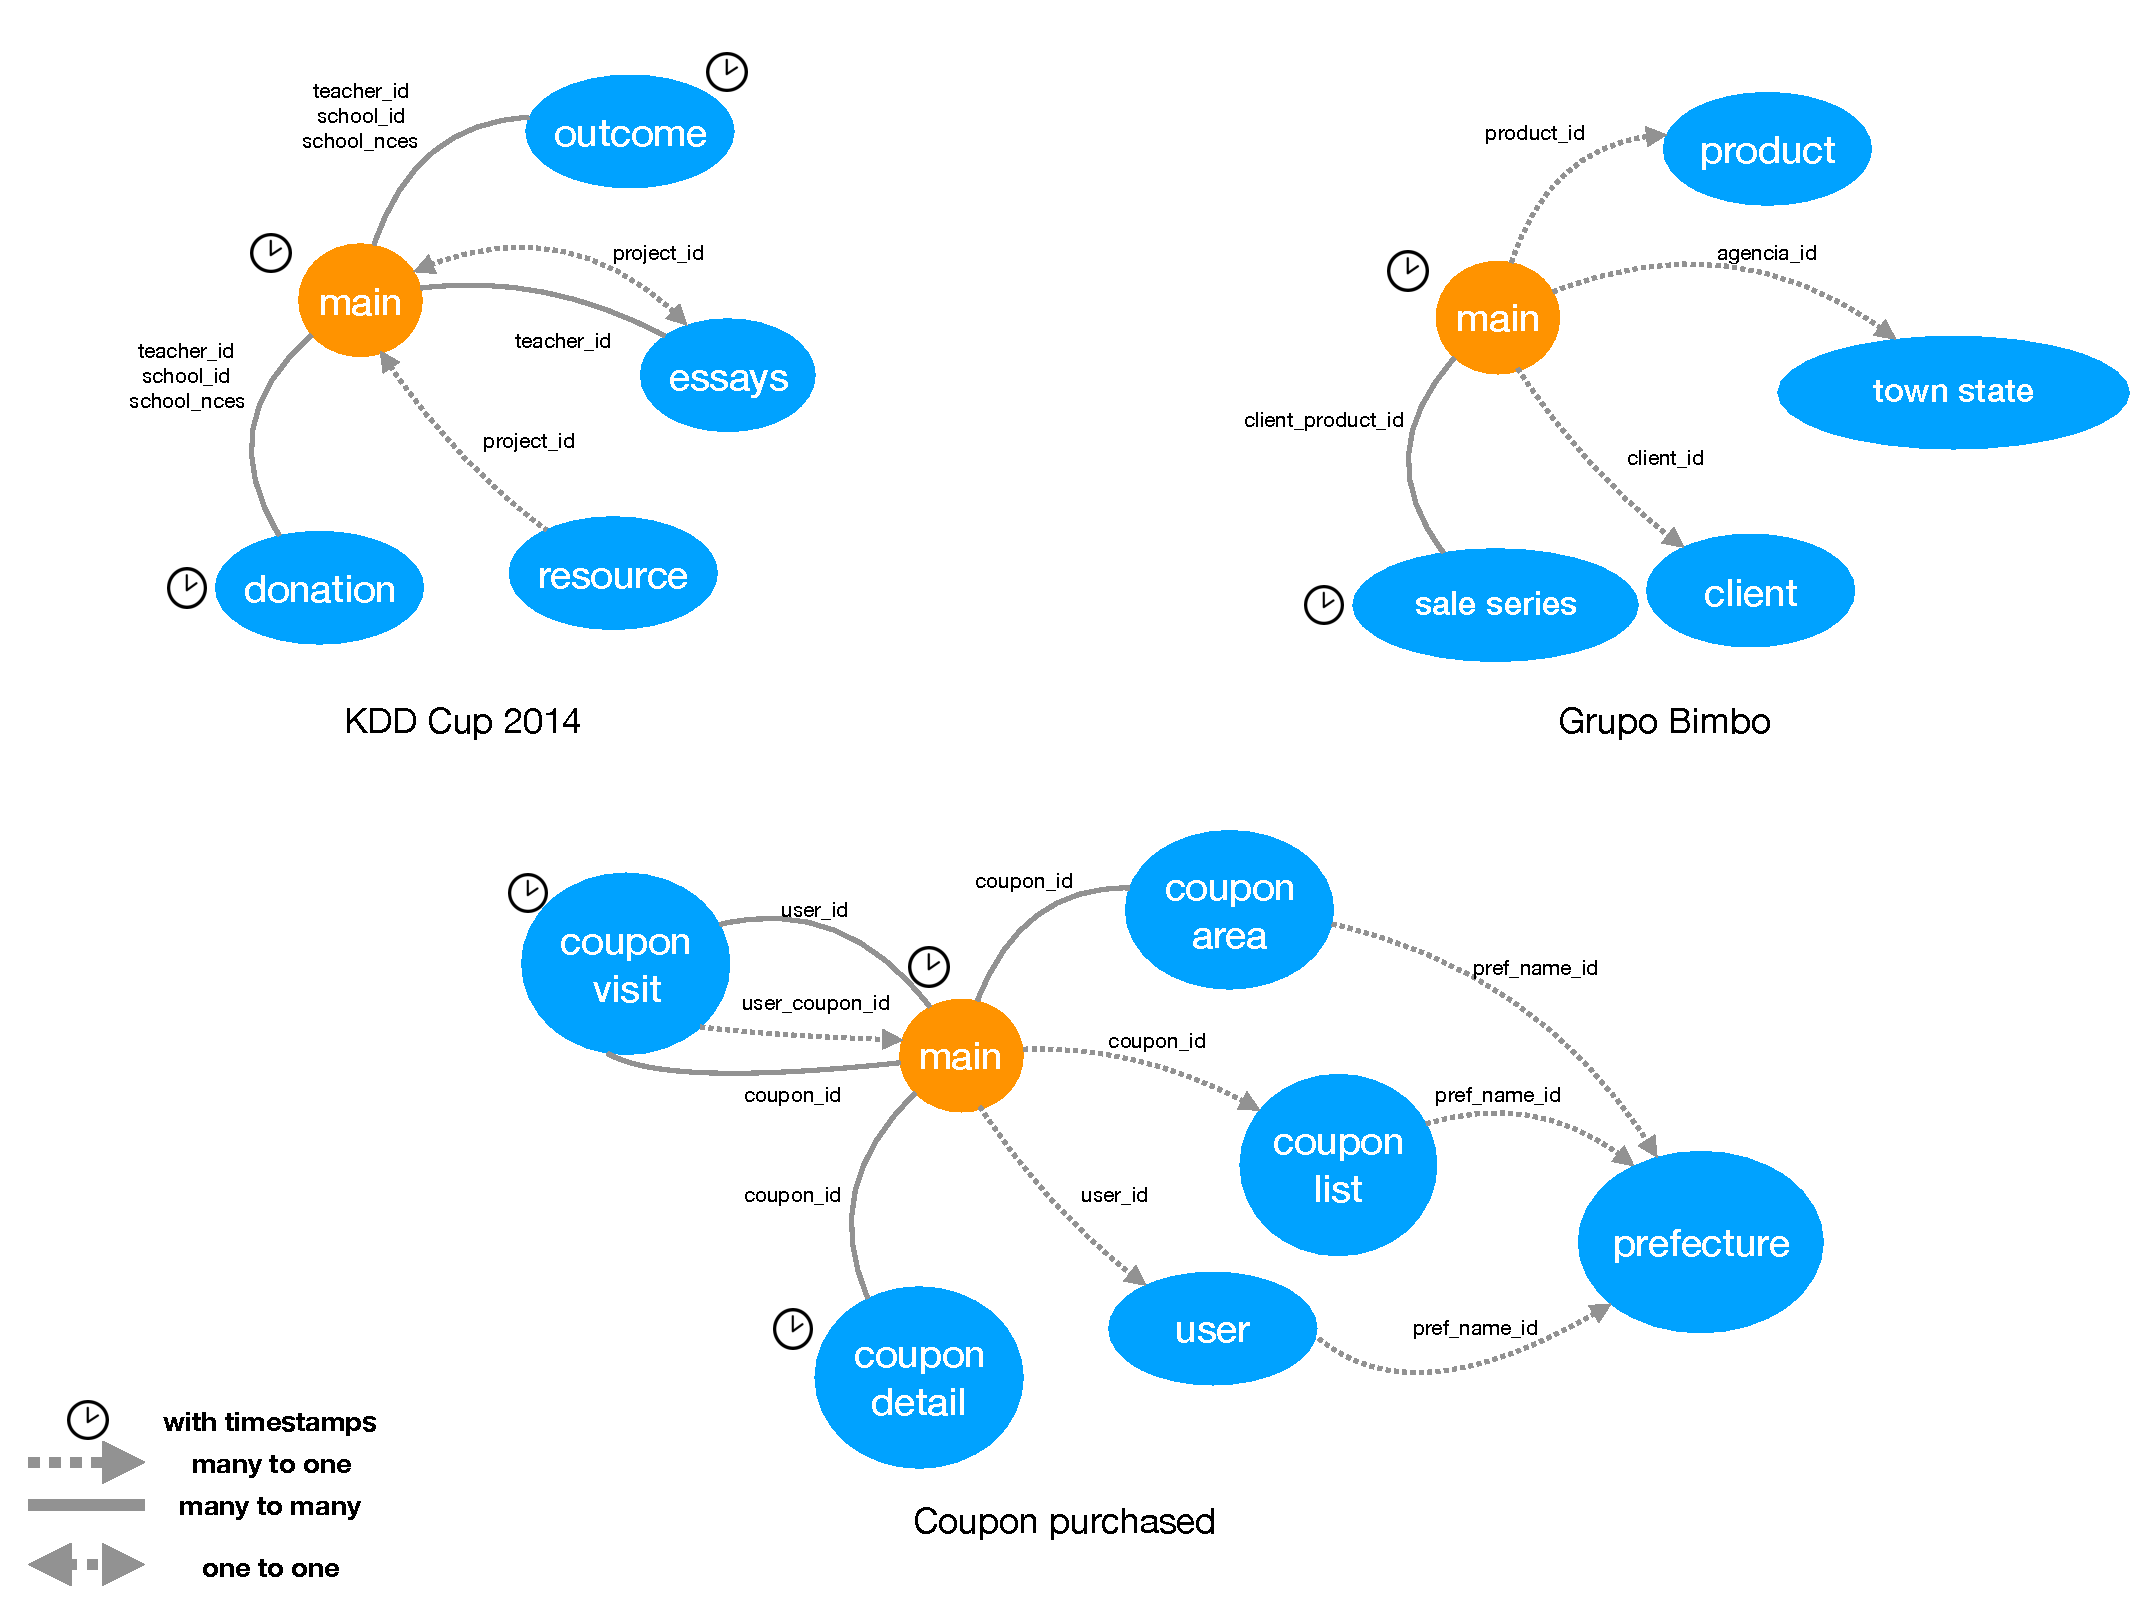
\includegraphics[width=1.0\textwidth]{./egraph.pdf}
    \caption{Entity graphs of the Kaggle datasets}
    \label{fig:kaggle database}
\end{figure*} 

\paragraph{KDD Cup 2014} participants were asked to predict which project proposals are successful based on their data about:
\begin{itemize}
\item \textit{projects}:   project descriptions, school and teacher profiles and locations. The project table is considered as the main table in our experiment as it contains the target column.
\item \textit{essays}: written by teachers who proposed the proposal as a project goal statement.
\item \textit{resources}: information about the requested resources
\item \textit{donation}:  historical donation information. The donation table in the competition  includes data for training but not for testing. Therefore, we ignored the donation table in the feature extraction process.
\item \textit{outcome}: historical outcome of the past projects. We add three missing key columns (school ID, teacher ID, school NCES ID) to the outcome table to connect it to the main table. This allows our system to explore the historical outcome for each school, teacher and school NCES ID.
\end{itemize} 
 The entity graphs of the datasets are shown in Figure \ref{fig:kaggle database}. In all datasets, we experimented with the forward only graph traversal policy. In the given policy, the maximum search depth is always set  to the maximum depth of the breadth-first search of the entity graph starting from the main table. 
 


\subsection{Experimental settings and running time}
A Spark cluster with 60 cores, 300 GB of memory and 2 TB of disk space was used to run the rule-based OneBM algorithm. Features from OneBM were fit into an XGBOOST model known as the most popular model in the Kaggle community. Hyperparameters of XGBOOST were auto-tuned via the Bayesian optimization described in section \ref{sec:tuning}. The maximum number of iterations in the hyperparameter auto-tuning algorithm was set to 50. There are several hyperparameters in OneBM feature extraction, these hyper-parameters were not tuned in our work but fixed to popular settings \cite{dlbook} in advanced as shown in Table \ref{tab:parameters}. 

To train the r2n networks, we used a machine with one GPU with 12 GB of memory and 4 CPU cores with 100 GB of memory. Training one model until convergence needed  7 days. Auto-tuning the r2n hyper-parameters with minimum 50 steps in three datasets would take 150 weeks. Therefore, we didn't consider auto hyper-parameter tuning   for r2n. The network structure hyperparameters are fixed as shown in Table \ref{tab:parameters} (see Appendix ) based on computational feasibility in our available computing resource. All results are reported based on the Kaggle private leaderboard ranking information. The running time of the algorithms is reported in Table \ref{tab:running time}. As can be observed, OneBM was scaling better than the other methods thanks to its parallel implementation in Spark.


\begin{table}
  \begin{center}
  \caption{Running time.} \label{tab:running time} 
  \begin{tabular}{ | l | c | c | c|}
    \hline
    \textbf{Data} & \textbf{OneBM} & \textbf{r2n}  & \textbf{DFS} \\ \hline
    Computing res. & 60 CPUs  & CPU + GPU& 1 CPU \\ \hline
    KDD Cup 2014 & 12.9 hours & one week&  NA \\ \hline    
    Coupon purchase &  2.8 hours &  one week&  84.04 hours \\ \hline 
    Grupo Bimbo &  56 min. &  1 week&  2 weeks \\ &&&(not finished) \\ \hline        	
  \end{tabular}
  \end{center}  
\end{table}

\subsection{Kaggle competition results and discussion}
\begin{table*}
  \begin{center}

  \caption{Performance of different methods on Kaggle competitions. Our methods including OneBM, r2n or their linear ensemble achieved two silver medals and one bronze medal. The results of DFS in KDD Cup 2014 was reported in \cite{DFS}}   \label{tab:results} 
  \begin{tabular}{ | l | c | l | l |l|l|}
    \hline
    \textbf{Data} & \textbf{Results} & \textbf{DFS} & \textbf{OneBM} & \textbf{R2N} & \textbf{Ensemble} \\ \hline
    & Ranking &  145/472 & 37/472  & 40/472  &\textbf{31/472}  \\ 
    KDD Cup 2014 & AUC &  0.586 &  0.622 & 0.619 & \textbf{0.626}  \\ 
    & Top \% &  30 &  7.8& 8.4 & \textbf{6.5} \\ 
    & Medals &  No &  \textbf{Silver} & \textbf{Silver} &  \textbf{Silver} \\ \hline
    & Ranking &  NA &  181/1969 & 312/1969 &  \textbf{152/1969}\\ 
    Grupo Bimbo & LRMSE &  NA &  0.475 & 0.485 &  \textbf{0.472}   \\ 
    & Top \% &  NA &  9.1 & 19.4 & \textbf{7.7} \\ 
    & Medals &  NA &  \textbf{Bronze} & No & \textbf{Bronze} \\ \hline
    & Ranking & 448/1076 &  \textbf{30/1076} & 712/1076\ & 90/1076 \\ 
    Coupon Purchase & MAP@10 &  0.005635 &  \textbf{0.007416} & 0.004228&  0.006065 \\ 
    & Top \% &  41 &  \textbf{2.7} & 66 & 8.3\\ 
    & Medals &  No &  \textbf{Silver} & No & Bronze \\ \hline
  \end{tabular}
  \end{center}
\end{table*}
We report the results of DFS, OneBM, r2n and a linear ensemble (with equal weights) of r2n and OneBM on three Kaggle competitions where results are available (the result of DFS on Bimbo was not available as its run didn't finish within time limit). Table \ref{tab:results} shows that in the KDD Cup 2014 competition, both OneBM and r2n outperformed DFS with a significant margin. OneBM always achieves  better results than r2n because of the robustness of the XGBOOST model which was auto-tuned by Bayesian optimization. We observed that r2n was quite sensitive to the network structures.  Searching for the optimal network structure is a computationally expensive problem which is  out of the scope of this work. However, r2n provides additional benefit to the rule-based approach  as the linear ensemble of these methods show better results than each individual model in both KDD Cup 2014 and Grupo Bimbo competitions. Overall, our methods achieved 2 silver and 1 bronze medals in these competitions. 
 
 \begin{figure*}[tb]
    \centering
    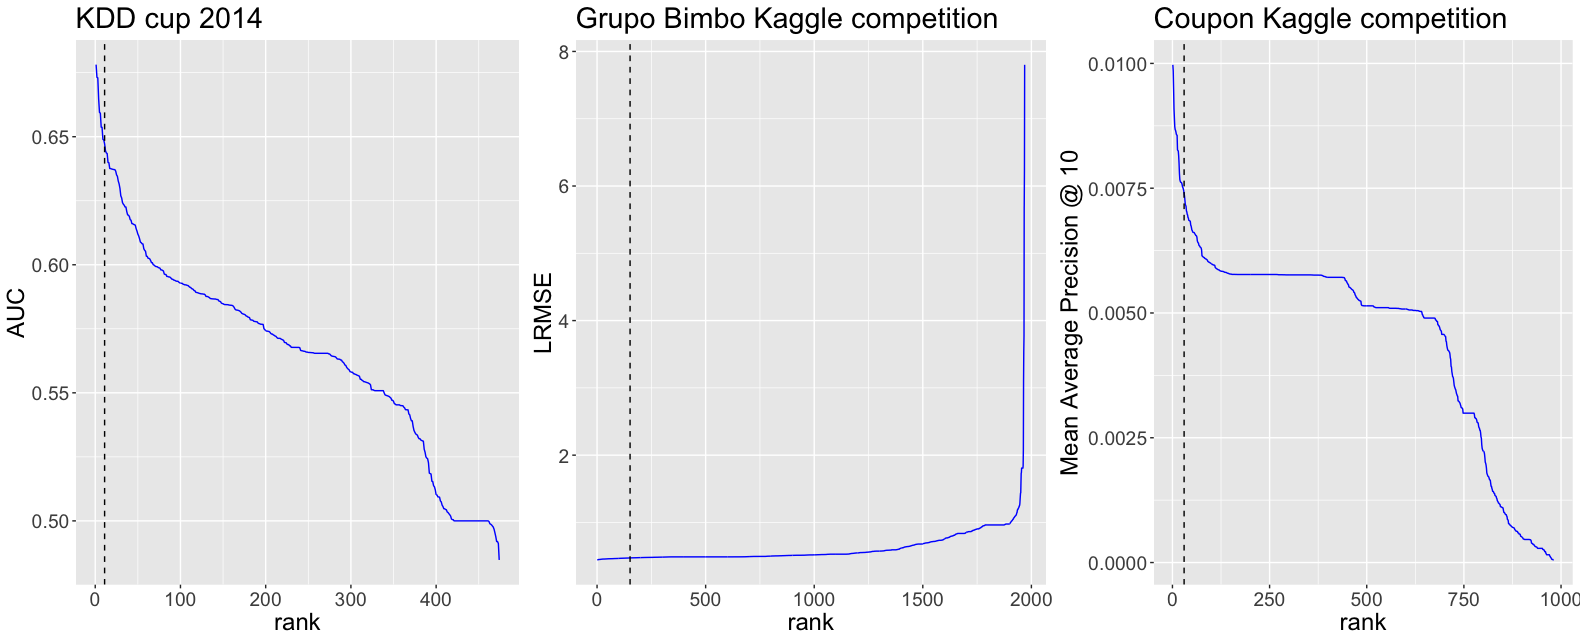
\includegraphics[width=1.0\textwidth]{./rank.png}
    \caption{Final results on the private leaderboard ordered by rank. Our hypothetical rank is depicted by a dotted line.}
    \label{fig:rank}
\end{figure*} 

Figure \ref{fig:rank} shows a comparison between our methods (best of OneBM, r2n and the linear ensemble marked with dotted line) and all Kaggle participants. As it is observed, in term of prediction accuracy, our method outperformed most participants and achieved results that were very close to the best teams. It is important to notice that each competition usually lasts for about two to three months. On the other hand, we achieved the results within one or two weeks whereas the feature engineering tasks were fully automated. In practice, data scientists work on many predictive analytics problems in parallel in a try-and-error manner until achieving the best analytics. Feature engineering is repeated many times in that cycle with different use-cases and data. Therefore,  our system will help data scientists save substantial time and efforts in an analytic project with minor trade-off for the best prediction results.   
\section{Related Work}
Automation of data science is a broad topic which includes automation of five basic steps: problem formulation, data acquisition, data curation, feature engineering, model selection and hyper-parameter tuning. Most related work in the literature focuses on the last two steps: \textit{automation of model selection, hyper-parameter tuning and feature engineering}. In the following subsections, related work regarding automation of these last two steps is discussed.
\subsection{Automatic model selection and tuning}
Auto-Weka \cite{kotthoff2016auto,ThoHutHooLey13-AutoWEKA} and Auto-SkLearn \cite{feurer2015efficient} are two popular tools trying to find the best combination of data preprocessing, hyper-parameter tuning and model selection. Both works are based on  Bayesian optimization \cite{brochu2010tutorial} to avoid exhaustive grid-search parameter enumeration. These works are built on top of existing algorithms and data preprocessing techniques in Weka\footnote{http://www.cs.waikato.ac.nz/ml/weka/} and Scikit-Learn\footnote{scikit-learn.org}, thus they are very handy for practical use.

Cognitive Automation of Data Science (CADS) \cite{cads,read} is another system built on top of Weka, SPSS and R to automate model selection and hyper-parameter tuning processes. CADS was made of three basic components: a repository of analytics algorithm with meta data, a learning control strategy that determines model and configuration for different analytics tasks and an interactive user interface. CADS is one of the first solutions deployed in industry. 

Besides the aforementioned works, Automatic Ensemble \cite{ensemble} is the most recent work which uses stacking and meta-data to assist model selection and tuning. TPOT \cite{tpot} is another system that uses genetic programming to find the best model configuration and preprocessing work-flow. Automatic Statistician \cite{autostatistician} is similar to the works just described but focuses more on time-series data and interpretation of the models in natural language.

In summary, automation of hyper-parameter tuning and model selection is a very attractive research topic with very rich literature. The key difference between our work and these works is that, while the state-of-the-art focuses on optimization of models given a ready set of features stored in a single table, our work focuses on preparing features as an input to these systems from relational databases with multiple tables. Therefore, these works are orthogonal to each other. In principle, we can use any system in this category to fine-tune the models with the input provided by OneBM.

\subsection{Automatic feature engineering}
Differently from automation of model selection and tuning where the literature is very rich, only a few works have been proposed to completely automate feature engineering for general problems. The main reason is that feature engineering is both domain and data specific. Therefore, we are distinguishing between automatic feature engineering for non-relational and relational data.

\subsubsection{Relational data }
Data Science Machine (DFS) \cite{DFS} is the first system that automates feature engineering from relational data with multiple tables.  DFS has been shown to achieve good results on  public data science competitions. A disadvantage of the DFS framework is that it does not support feature learning for unstructured data such as sets, sequences, series, text and so on. Features extracted by DFS are basic statistics which were aggregated for every training example independently from the target variable and from other examples. In many cases, data scientists need a framework where they can perform feature learning from the entire data collection and the target variable. Moreover, for each type of unstructured data, the features are beyond simple statistics. In most cases, they concern important structure and patterns in the data. Searching for these patterns from structured/unstructured data is the key role of data scientists. Therefore, in this work we extend DFS to a framework that allows data scientists to perform feature learning on different kinds of structured/unstructured data. 

Our work shares common points with  Inductive Logic Programming and Statistical Relational Learning (StarAI) \cite{lisa}. StarAI also focuses on finding patterns over multiple tables or informative joint features. The most related work in this topic is wordification \cite{wordification}. Wordification discretises the data into words from which the joined results can be considered as a bag of words. Each word in the bag can be considered as a feature for further predictive modeling. Similar to DFS and OneBM, wordification is a rule-based approach. It produces a lot of features irrespective of the target variable. Moreover, it does not support temporal data and unstructured data such as texts, images or sequences.
 

\subsubsection{Non-relational data }
Cognito \cite{cognito}  automates feature engineering for one table. It applies recursively a set of predefined mathematical transformations on the table's columns to obtain new features from the original data. Cognito improved prediction accuracy on UCI datasets. Since it does not support relational databases with multiple tables and is orthogonal to our approach and the DFS system, we do not compare to Cognito. 

\section{Conclusion and future work}
In this work, we have shown that feature engineering for relational data  can be automated using predefined sets of heuristic transformations or by the r2n network structure. The experiment results on three different Kaggle competitions showed very encouraging prediction in comparison to hand-crafted features extracted by top data scientists. By trading off a small prediction accuracy compared to the best results, but equivalent  to top 3-8\% best results, data scientists can save plenty of time in a data analytics project and be more productive.    

Our work opens many interesting research problems that are worth investigated in the future. First, the r2n network structure in this work is not auto-tuned due to efficiency issue. Future work should focus on efficient methods for network structure search to  boost the current results even more. Second, the rule based approach seems to be the best choice so far because of its effectiveness and efficiency, yet there are chances to improve the results further if a smarter graph traversal policy is considered. Although we proved that finding the best joining path is NP-hard, the theoretical analysis assumes that there is no domain knowledge about the data. We believe that exploitation of semantic relation between tables and columns can lead to better search algorithm and better features.  




\bibliographystyle{ACM-Reference-Format}
\bibliography{sigproc}

\pagebreak
\pagebreak
\newpage
\newpage
\begin{appendices}
\section{Proof of Lemma \ref{lemma:set function rnn} }
Denote $s$ as a set of numbers and $p(s)$ is any random permutation of $s$. A set function $f(s)$ is a map from any set $s$ to a real-value. Function $f$ is invariant with respect to set-permutation operation, i.e. $f(s) = f(p(s))$. For simplicity, we prove the lemma when the input is a set of scalar numbers. The general case for a set of vectors is proved in a similar way.


Consider the special case when $s = \{x_0, x_1\}$ and $p(s) = \{x_1, x_0\}$. According to definition of recurrent neural net we have:
\begin{eqnarray}
h_t &=& b + H*h_{t-1} + W*x_t \\ 
o_t &=& c + U*h_t
\end{eqnarray}

from which we have $rnn(s) = o_2$, where:
\begin{eqnarray}
h_1 &=& b + H*h_0 + W*x_0 \\
o_1 &=& c + U*h_1 \\
h_2 &=& b + H*h_1 + W*x_1 \\
o_2 &=& c + U*h_2 
\end{eqnarray}

In a similar way we can obtain the value of $rnn(p(s)) = o^*_2$, where:
\begin{eqnarray}
h^*_1 &=& b + H*h^*_0 + W*x_1 \\
o^*_1 &=& c + U*h^*_1 \\
h^*_2 &=& b + H*h^*_1 + W*x_0 \\
o^*_2 &=& c + U*h^*_2 
\end{eqnarray}
Since $rnn(p(s)) = rnn(s)$, we infer that:
\begin{eqnarray}
U*(H-1)*W *(x_0-x_1) = 0
\end{eqnarray}
The last equation holds for all value of $x_0, x_1$, therefore, either $H=1$, $W=0$ or $U=0$. The lemma is proved.
\section{Efficient implementation on GPU}
Deep learning techniques takes the advantage of fast matrix computation capabilities of GPU to speed up its training time. The speed-up is highly dependent upon whether or not the computation can be packed into a fixed size tensor before sending it to GPUs for massive parallel matrix computation. A problem with the network is that the structures of relational trees are different even for a given joining path. For instances, the relational trees in Figure \ref{exp:relational tree} have different structures depending on input data. This issue makes it difficult to normalize the computation across different relational trees in the same mini-batch to take the advantage of GPU computation. 

In this section, we discuss a computation normalization approach that allows speeding up the implementation 5x-10x using GPU computation under the assumption that the input to an r2n network are relational trees we set $\{D_{p_1}, D_{p_2}, \cdots, D_{p_q} \}$, where $D_{p_i} = \{t^{p_i}_1, t^{p_i}_2, \cdots, t^{p_i}_m\}$. 

It is important to notice that $t^{p_k}_i$ and $t^{p_l}_i$ have different structure when $p_l$ and $p_k$ are different. Therefore, normalization across joining paths is not a reasonable approach. For a given joining path $p_i$, the trees $t^{p_i}_k$ and $t^{p_i}_l$ in the set $D_{p_i}$ may have different structures as well. Fortunately, those trees share commons properties:
\begin{itemize}
\item they have the same maximum depth equal to the length of the path $p_i$
\item transformation based on RNN at each depth of the trees are shared
\end{itemize} 

Thanks to the common properties between the trees in $D_{p_i}$ the computation across the trees can be normalized. The input data at each depth of all the trees in $D_{p_i}$ (or a mini-batch) are transformed at once using the shared transformation network at the given depth. The output of the transformation is a list, for which we just need to identify which output corresponds to which tree for further transformation at the parent nodes of the trees.
 
 
\section{Model hyper-parameter tuning with Bayesian optimization }
The quality of the prediction highly depends on various hyper-parameters present in the machine learning method. Since their optimal choice highly depends on the data, fixing them abitrarily will provide suboptimal results. Therefore, we make use of Bayesian optimization \cite{Mockus1975}, a state-of-the-art approach for efficient and automated hyperparameter optimization \cite{Snoek2012}.

For Bayesian optimization, the problem of hyperparameter optimization is formulated as a black-box function minimization problem.  We define this black-box function $f$ by
\begin{equation}
f\ :\ \Lambda\rightarrow\mathbb{R}\enspace,
\end{equation}
where $f$ maps a hyperparameter configuration $\boldsymbol{\lambda}\in\Lambda$ to its loss on the validation data set. The evaluation of $f$ is a time-consuming step because it involves training our neural network on the training data set and evaluating it on the validation data set. However, minimizing $f$ will provide us the optimal hyperparameter configuration. 
\begin{equation}
\boldsymbol{\lambda}^{\ast}=\underset{\boldsymbol{\lambda}\in\Lambda}{\arg\,\min}f\left(\boldsymbol{\lambda}\right)\enspace.
\end{equation}

Bayesian optimization efficiently minimizes this expensive black-box function sequentially. In each optimization iteration the function $f$ is approximated by a Bayesian machine learning model, the surrogate model. We selected a Gaussian process with Mat\'{e}rn $\sfrac{5}{2}$ kernel as our surrogate model. This Bayesian model provides point and uncertainty estimates for the whole hyperparameter search space. According to a heuristic considering both mean and uncertainty prediction, the most promising hyperparameter configuration is evaluated next. We select expected improvement as our acquisition function \cite{Mockus1975}.
\label{sec:tuning}
\section{Parameter settings}
See Table \ref{tab:parameters}
\begin{table}[h]
  \small
  \begin{center}
  \caption {Parameter settings for OneBM and the r2n networks} \label{tab:parameters} 
  \begin{tabular}{ | l | c | }
   
    \hline
    \textbf{parameter} & \textbf{value} \\ \hline
    The number of recent values &  10  \\ \hline
    Maximum joined table size & $10^9$  \\ \hline
    The number of  highest correlated items & 10 \\ \hline
    Min correlation & $10^{-16}$ \\ \hline
    Min info-gain & $10^{-16}$ \\ \hline
    Optimization algorithm for backprop & ADAM \\ \hline
    Learning rate of ADAM & 0.01 \\ \hline
    Initial weights for FC and feed-forwards & Xavier \\ \hline
    Output size of FCs & 10 \\ \hline
    The number of  hidden layers in feedforward layers & 1 \\ \hline
    The number of  hidden layer size in feedforward layers & 1024 \\ \hline
	RNN cell &  LSTM \\ \hline
	LSTM cell size & 18 \\ \hline
	Max input sequence size & 50 \\ \hline
	Early  termination after no improvement on & 25\% training data \\ \hline
	Validation ratio & 10\% training data \\ \hline
  \end{tabular}
  \end{center}
\end{table}
\begin{figure*}[tb]
    \centering
    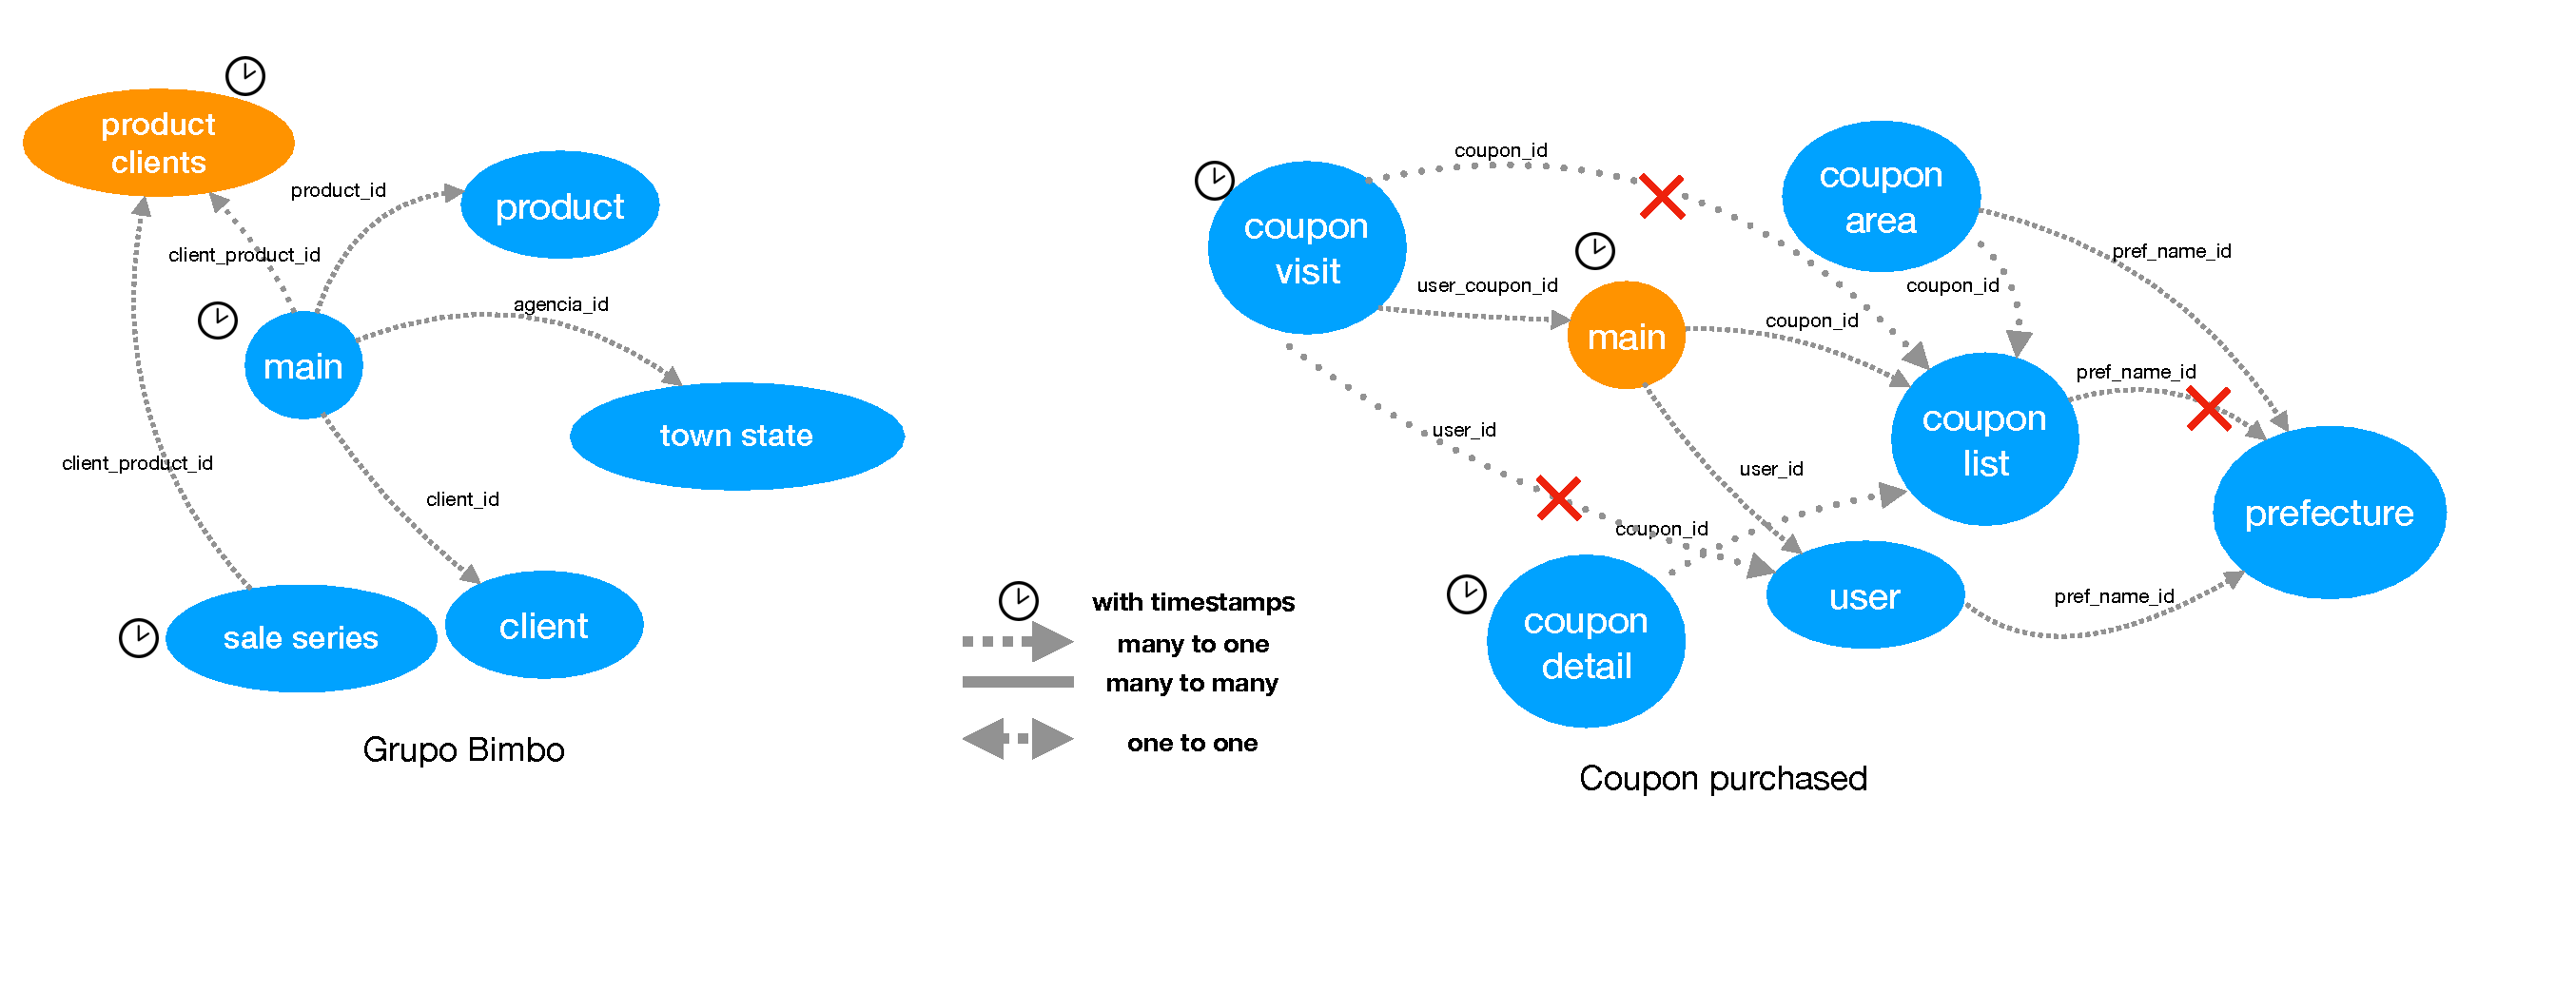
\includegraphics[width=1.0\textwidth]{./egraph_copy.pdf}
    \caption{Tweaked entity graphs of the Kaggle data used in our experiments for DFS}
    \label{tweak-database}
\end{figure*} 
\section{Baseline method settings}
DFS is  currently considered as the state of the art for automation of feature engineering for relational data. Recently,  DFS was  open-sourced\footnote{https://www.featuretools.com/} .  We compared OneBM and r2n to DFS (version 0.1.14). It is important to notice that the open-source version of DFS has been improved a lot since its first publication \cite{DFS}. For example, in the first version described in the publication there is no concept of temporal index which is very important to avoid mining leakages.

In order to use DFS properly, it requires knowledge about the data to create additional tables for interesting entities and to avoid  creating diamond entity graphs because DFS doesn't support diamond loops in the graph and does not allow many-many relations. The results of Grupo Bimbo and Coupon purchase competitions were reported using the open-source DFS after consulting with the authors on how to use DFS properly on these datasets.

For the Bimbo and Coupon purchased data, the entity graphs shown in  Figure \ref{fig:kaggle database} are not supported by DFS as they contain many-many relations and diamond subgraphs. Therefore, we  tweaked these graphs to let it run under the DFS framework. Particularly, for Bimbo data the relation between main and series tables is many-many. To go around this problem,  we created an additional table called product-client from the sale series table. Each entry in the new table   encodes the product, client pairs.  The product-client is the main table correspond to product-client pair. Since the competition asked for predicting sales of every pair of product-client at different time points, we created a cut-off time-stamp table, where each entry corresponds to exactly one  cut-off timestamp. The new entity graph is presented in Figure \ref{tweak-database}. We run DFS with maximum depth set to 1 and 2 and 3.

For Coupon datasets, more efforts are needed to prepare a proper input for DFS because the original entity graph contains both diamond loops and many-many relations. The latter issue can be resolved  by changing the connections as demonstrated in Figure \ref{tweak-database}. To avoid diamond loops we need to delete some relations. We decided to delete the relations (marked with an X) in Figure \ref{tweak-database}. Alternatively, we also tried to delete the relation between the  main and coupon-visit table but that led to much worse prediction than the given choice. 

In general, the results are highly dependant on how we use the tool so for the KDD cup 2014,  to have a fair comparison, we used the results in the original publication \cite{DFS}.  For KDD Cup 2015 and IJCAI 2015, the competitions are closed for submissions so  we couldn't report the results.

\section{Acknowledgements}
We would like to thank Johann Thiebaut, Dr. Tiep Mai, Dr. Bei Chen, Dr. Oznur Alkan, Dr. Olivier Verscheure, Dr. Eric Bouillet, Dr. Sean McKenna, Dr. Pol McAonghusa, Dr. Horst C. Samulowitz, Dr. Udayan Khurana and Tejaswina Pedapat for useful discussion and support during the development of the project.  We would like to thank Max Kanter for explaining us how to use DFS (featuretools) for the experiments.


\end{appendices}



\end{document}
